\documentclass[USenglish,letterpaper,12pt,extrafontsizes,oneside,onecolumn,final]{memoir}

\usepackage{babel}
\usepackage[minionint,mathlf]{MinionPro}
\renewcommand{\sfdefault}{Myriad-LF}
\usepackage{inconsolata}
\usepackage{pifont} % for Dingbats
\usepackage{lettrine} % for dropped capitals
\usepackage[babel=true,protrusion=true,expansion=true,kerning=true,spacing=true,tracking=true]{microtype}
\usepackage{graphicx,color}
%\usepackage{array}
\usepackage{xspace}
\usepackage[numberedbib,bibnewpage,nosectionbib,tocbib]{apacite}
\usepackage{tabulary}
\usepackage{amsmath}

\nonzeroparskip % this chooses a good space between paragraphs
%\setlength{\parindent}{0pt} % paragraph indentation amount
\OnehalfSpacing % line spacing command
%\DoubleSpacing
%\setSingleSpace{1.05} 
\setDisplayskipStretch{0.05} % increasing spacing around math displays

% these commands help avoid widow and orphan lines from paragraphs
\clubpenalty=10000
\widowpenalty=10000
\raggedbottom	
%\sloppybottom

% to make ligatures searchable
% the file glyphtounicode.tex can be in the same directory 
% as the main tex file or in the local latex file directory
\input{glyphtounicode}
\pdfgentounicode=1

\newcommand{\deltap}{$\Delta P$}

% I will decide later what sort of style to use
%\chapterstyle{chappell}
\headstyles{dowding}

% This sets the spine and edge margins
\setlrmarginsandblock{1.5in}{1.5in}{*}
\checkandfixthelayout

\title{\textsc{The Illusion of\\the Illusion of Control}}
\author{\textsc{Zachariah S. Sharek}}
\date{}
\pretitle{\begin{flushright}\LARGE}
\posttitle{\par\end{flushright}\vskip 4em}
\preauthor{\begin{flushright}\LARGE}
\postauthor{\par\end{flushright}\vskip 0.5em}
\setlength{\droptitle}{3cm}

\begin{document}

\frontmatter
%\begin{titlingpage}
\maketitle
\thispagestyle{empty}
\clearpage
%\end{titlingpage}

\begin{flushright}
\textit{For my father\\who always encouraged me}
\clearpage
\end{flushright}

\begin{center}
\Large\textbf{Acknowledgements}\\
\end{center}
I am grateful for the support, encouragement and guidance that I received from my committee of Don Moore, Francesca Gino and Laurie Weingart.  I have benefited tremendously from the advice I have received from them during my time at Carnegie Mellon.  I especially appreciate my adviser, Don Moore, and his patience and enthusiasm for my work. 

I also thank the rest of the faculty in the Organizational Behaviour department at Tepper for their feedback and advice, Mark Fichman, in particular has been quite helpful and encouraging.  I have also benefited from and thoroughly enjoyed my discussions with Jack Stecher and his contagious enthusiasm. This dissertation has also benefited from comments and advice by Teddy Seidenfeld, Jay Kadane and Joachim Vosgerau.  I also appreciate the help I received from Alan Scheller-Wolf and Susan Ambrose and the always cheerful assistance from Lawrence Rapp.   

Daylian Cain has been a wonderful friend over the years and it was mainly due to his encouragement that I started this journey.  I appreciate his advice and generosity but most of all I especially value his friendship.

I have been richly blessed to have a supportive and loving family.  My mother, Catherine Sharek, has always given excellent advice and for this dissertation has been especially generous with her time in reading it and providing valuable comments.  My brother and sister, David and Lisa Sharek, have always been encouraging and generous.  David spent a tremendous amount of time helping me with code and advice, never asking for anything in return.  I am also thankful for the support and encouragement from my fianc\'{e}e's family, especially Linda and Frank Hooper.  

Finally, and most importantly, my fianc\'{e}e, Danielle Hooper, has been a saint to me over the last few years, putting up and caring for me with love and patience. I don't know how she did it.  I can't wait until June 9th!

\clearpage

% These commands set the abstract title and text font formats 
\renewcommand{\abstractnamefont}{\Large\bfseries}
\renewcommand{\abstracttextfont}{\normalfont}

\begin{abstract}
This dissertation is an exploration of people's estimates of control, with a particular focus on the \emph{illusion of control}.  Ellen Langer's 1975 article introduced the illusion of control as ``an expectancy of a personal success probability inappropriately higher than the objective probability would warrant.''  Since her work, subsequent research has focused on factors, such as mood, intention, and connection to the outcomes that modify estimates of control, but little work has been done to investigate the \emph{process} by which people estimate control.  The studies presented here---six experimental and one simulation---address this gap.  

My central question is: \emph{Are people's estimates of control accurate?} The consideration of this question raises further questions that have not been deeply explored in the illusion of control literature.  For example, how can we judge the accuracy of people's estimates of control?  Are laypersons' definitions of control congruent with a normative standard for accuracy?  What is the process by which people estimate control and can we model this?  Can we extend our examination of control into domains where outcomes are not dichotomous?

I address the constancy of the illusion of control by examining how people estimate control in situations where their objective control is high.  Two studies using a novel paradigm show that people under-estimate control when it is objectively high and over-estimate it when control is objectively low.  A third study using a common illusion of control experimental design, the event-onset paradigm, replicates this finding.  Together, these three studies question whether people have an innate bias towards believing they have more control than they really do.  

But just how do people estimate control?  To address this question, I develop a normative model for estimating control using a widely accepted normative measure of control. Based on the results of the first three studies, this model is simulated being used by a pool of perfectly Bayesian reasoners. The simulation results yields final estimates of control extremely similar to experimental estimates, indicating that this model accurately captures some of the process people use to estimate control.  The simulation results are also statistically significant when compared to the objective amount of control in the simulation when frequentist (i.e. Fischer-Pearson) statistical tests are used.  Significant results implies that these perfect Bayesian agents are inaccurate when judged by the standard statistical norms, yet Bayesian inference is widely accepted as a normative method of assimilating information!  These results indicate a possibly serious methodological issue with many experimental paradigms that rely on standard statistical tests when measuring information learning.  

Next, similar themes are pursued experimentally, when a novel method of eliciting estimates of contingency during an event-onset experiment and the participant responses afterwards demonstrate that, contrary to conventional beliefs, people are quite accurate at estimating contingency (and performing information processing in a Bayesian manner), yet their estimates of control still follow the familiar pattern of results shown in the first three studies.  This implies that participants' definitions of control are sharply at odds with the experimental normative measure of control. Thus, the illusion of control (and mis-estimates of control in general) might be experimental artefacts due to a failure to ensure that the concept of control is agreed upon by both experimenters and participants.  A subsequent study replicates these results even when participants' estimates of contingency are not elicited during the experiment--and potentially less salient--and participants are free to sample as little or as long as they wish.  

Finally, the examination of estimates of control is taken beyond the dichotomous realm of success or failure and into situations where outcomes can vary along a scale, for example, when a stock price goes up or down by a variable amount.  The previous normative measure of control is extended into these domains and tested in an experimental setting when participants are able to evaluate their actions against the number of widgets produced in a factory.  The results show again, that people are good at estimating contingencies, yet fail to incorporate them into a normative manner when asked to estimate control.  

The results of the studies in this dissertation reveal that the illusion of control, along with mis-estimates of control in general, appears to be an illusion itself due to a lack of common understanding of how control should be calculated. These results are replicated across several different paradigms and appear to be robust.  Additionally, these studies reveal methodological issues with previous work on the illusion of control and suggest that greater care needs to be taken when examining concepts whose measurement is not obvious. So are people's estimates of control accurate? My work shows that, yes, people are accurate when they estimate control, but only if you ask them properly.
\end{abstract}
\clearpage

\tableofcontents*
\clearpage

\mainmatter
\chapter{Introduction}
\label{chap:intro}

\setlength{\epigraphwidth}{18em}
\epigraphfontsize{\footnotesize}

\epigraph{\SingleSpacing Nature has kept us at a great distance from all her secrets, and has afforded us only the knowledge of a few superficial qualities of objects; while she conceals from us those powers and principles on which the influence of those objects entirely depends.}{\textit{An Enquiry Concerning Human Understanding}\\ \textsc{David Hume}}

\lettrine[lines=2,slope=-3pt,nindent=2pt]{I}{n} the 1970s, the city of New York installed buttons at intersections with traffic lights. Helpful signs instructed pedestrians, ``To cross street, push button. Wait for walk signal.'' Since then, pedestrians in New York routinely have assumed that pushing the button speeds the arrival of the walk signal. As it happens, their faith is misplaced. Since the late 1980s, traffic signals in New York have been controlled by a computer system that determines when the walk signal is illuminated (Luo, 2004). Pushing the button has no effect. But because the city has not paid to remove the signs or the buttons, pedestrians continue to push the buttons. 

According to Langer (1975; Langer \& Roth, 1975), when people behave as if they have control in situations that are actually determined by chance (i.e., situations where they have no actual control), they are suffering from what she termed the ``illusion of control''. Many studies have shown that when cues related to skills, such as choice, competition, practice, or familiarity, are introduced into chance situations, people behave as if the chance outcome was determined by skill (Goffman, 1967; see also Thompson, Armstrong, \& Thomas, 1998 for a thorough review). For instance, choice has been shown to induce an illusion of control. People behave as if they think they have greater control when they roll dice themselves than when someone else rolls for them (e.g., Fleming \& Darley, 1986). People prefer to pick their own lottery numbers than to have others pick for them (Dunn \& Wilson, 1990; Langer, 1975). And pedestrians in New York City push the walk button even though it will not get them across the street any faster.

This dissertation is an exploration of people's estimates of control. Its central question is: \emph{Are people's estimates of control accurate?} The consideration of this question raises further questions that have not been deeply explored in the illusion of control literature.  For example, how can we judge the accuracy of people's estimates of control?  Are lay-persons' definitions of control congruent with a normative standard for accuracy?  
What is the process by which people estimate control and can we model this?  Can we extend our examination of control into domains where outcomes are not dichotomous?

The ensuing chapters examine these questions and others and are set out as follows:  Chapter \ref{chap:history}, \emph{\titleref{chap:history}}, reviews important aspects of previous work on the illusion of control and related research and examines a normative standard for measuring control.  This normative measure is then used, along with the results of previous research, to develop a normative model of the process of how estimates of control are created. Chapter \ref{chap:ioc}, \emph{\titleref{chap:ioc}}, presents three studies that challenge the assumption that people consistently over-estimate control by demonstrating that people under-estimate control when it is objectively high as well as over-estimating control when it is objectively low. The results from these studies and the normative results from chapter \ref{chap:history} are used in chapter \ref{chap:model}, \emph{\titleref{chap:model}}, to construct a Bayesian model which is tested via simulation, the outcomes of which compare favourably with previous experimental results. \emph{\titleref{chap:bioc}}, chapter \ref{chap:bioc}, builds on the success of this model to show that people's estimates of control could be the result of a definitional disparity of control between experimenters and participants.  The next chapter, \emph{\titleref{chap:explore}}, addresses possible alternative explanations for this result as well as gauging how people respond when presented with the normative measure of control discussed in chapter \ref{chap:history}.  The final study, \emph{\titleref{chap:widgets}}, in chapter \ref{chap:widgets} extends both the illusion of control experimental paradigm and a normative measure of control to situations where outcomes are non-dichotomous.  For example, how can you measure control when the results of your actions can be measured over a range of possible values, such as, with stock prices or a factory's output? This chapter presents a solution to this question and demonstrates that, consistent with the results from chapters \ref{chap:bioc} and \ref{chap:explore}, people's estimates of control tend towards accuracy if the right questions are asked. Finally, chapter \ref{chap:conclusion} concludes with a discussion of the results of these new studies and considers their impact, limitations and the future research possibilities they open up.

\chapter{On Control and its Illusions}
\label{chap:history}

\epigraph{\SingleSpacing As it is by means of thought only that any thing operates upon our passions, and as these are the only ties of our thoughts, they [the principles of association] are really to us the cement of the universe, and all the operations of the mind must, in a great measure, depend on them.}{\textit{A Treatise of Human Nature}\\ \textsc{David Hume}}

\section{Experimental Paradigms}

\lettrine[lines=2,slope=-3pt,nindent=2pt]{T}{he} idea that people systematically overestimate their control of events was introduced by Langer (1975), who defined the illusion of control as ``an expectancy of a personal success probability inappropriately higher than the objective probability would warrant.''  Langer showed the presence of cues usually associated with skill-based situations can induce people into believing that they exercise more control over a chance based situation than they really do.  Crucially, these experiments only examined pure chance situations, such as lottery tickets or trying to draw a high card from a deck; Langer did not examine estimates of control in situations where people actually had control. 

While the illusion of control is perceived as accepted fact that can be applied to human behavior in general (Thompson, 1999), this knowledge appears limited to awareness that people systematically overestimate their control, for example: ``People substantially overestimate their degree of control over heavily chance-determined events.'' (Taylor \& Brown, 1988, p. 196) and ``Because judgments that one can control the environment are often so pervasive, they may generalize to uncontrollable situations.'' (Presson and Benassi, p 493, 1996).   As pervasive and accepted the phenomenon of the illusion of control is, it is perhaps odd that little work has been done in broadening the scope of its research.  Skinner's comprehensive overview of constructs of control mentions the illusion of control in passing, mainly by briefly defining it as ``... people  have high perceived control in objectively uncontrollable or chance-determined situations'' (1996). This rigid perception of the definition of the illusion of control is perhaps the reason why the scope of work on the illusion of control has been limited. If the illusion of control can only be applied to non-contingent events, then, by definition, its application to the broader world outside of chance events is precluded.

Studies on the illusion of control have relied primarily on two paradigms. The first manipulates factors that the authors predict will influence perceptions of control (e.g., choice or familiarity) in a gambling game (e.g., dice throw). In these studies (e.g. Langer, 1975), participants are asked to bet money on the chance outcome or rate their confidence in a successful outcome. That is, they are asked to judge their control indirectly while they are attempting to execute control (e.g., roll a die). Thus, this paradigm involves no feedback for participants, one-shot tasks, and uses participants' predictions about the outcome of the task to measure control. 

Therefore, it is not surprising that prior research that used this paradigm has focused on people's estimates of control over heavily chance-determined events and not on examining people's assessments of control in situations where actual control is high. However, these situations are quite common in organizations and broader society more generally, and they often involve high--stake consequences --- such as stopping a car by stepping on the brake, working hard to increase one's odds of being promoted, or exercising in order to lose weight. Are people's estimates of their control accurate in these situations?  While Langer's use of this paradigm invigorated study into individual's assessments of control, its use of pure or almost pure-chance events limited experimental manipulations towards answering this question.  

In the second type of paradigm, the event-onset design (Jenkins and Ward, 1965; Alloy and Abramson, 1979; Alloy and Abramson, 1982), participants are told that they are to decide whether or not to perform an action (usually pressing a button) and observe the outcome over repeated trials, with the goal of discerning how much control their actions have on the onset of a particular event.\footnote{The event-onset design pre-dates Langer's work and was developed by Jenkins and Ward to study estimates of \emph{contingency}.} Studies using this second paradigm measure control by asking participants to estimate their degree of control over the task outcome. This paradigm involves feedback for participants in each round (by pressing the button, they receive feedback on whether it produces an outcome or not) and a measure of control that is based on past behavior. Additionally, this design allows for a variety of modifications such as adding more possible actions (cf. Jenkins and Ward, 1965, which presented participants with two buttons) and the experimental manipulation of the probabilities of an event occurring when action was and was not taken.  Thus, the adaptation of this allowed the illusion of control to be studied in contexts where participants had varying amounts of control.

\subsection{Event-onset research}
 
Previous illusion of control research using the event-onset paradigm has shown that there is a considerable disconnect between the objective control participants experienced and their subjective measure of control.  For instance, Jenkins and Ward's (1965) results showed that participants' subjective control was highly (and solely) correlated with the number of successful trials they observed and uncorrelated with the actual degree of control they observed. The overall success rate across all options is the average rate of success that a participant would experience and is called the \emph{reinforcement} rate. Jenkins and Ward did not offer an explanation for the process by which participants arrived at their estimates beyond noting these correlations implied that their participants did not have an abstract understanding of statistical contingency. 

According to Seligman's (1975) work on the learned helplessness theory of depression, depressed people believe they are ineffective and powerless to control what happens to them. It follows that depressed individuals should underestimate their control; Langer (1975) postulated that the illusion of control was the inverse of learned helplessness. Alloy and Abramson (1979, 1982) used the even-onset paradigm to test this theory by examining the differences in estimates of control between depressed and nondepressed participants. Their findings suggested, surprisingly, that depressed participants were more accurate in their estimates of control, whereas nondepressed participants overestimated their control.   

However, subsequent research suggested that depressed individuals simply report believing that they lack control, whereas nondepressed individuals report being in control (Dykman, Abramson, Alloy, \& Hartlage, 1989). As noted by Dykman et al. (1989), depressives perceive themselves to have less control than do nondepressives; as a result, depressives may appear accurate on uncontrollable tasks and inaccurate on controllable tasks.  The opposite is true for nondepressives. These findings suggest that accuracy or inaccuracy of perceptions of personal control is an accident of the match between an individual difference (i.e., depression) and task characteristics (i.e., actual difficulty or controllability). The factors that influence perceptions can move independently of the factors that influence objective performance, and accuracy depends on both.

There have been other early event-onset studies on factors affecting judgements of control such as Gollwitzer and Kinney (1989), who examined how motivational mind-sets, such as deliberative (pondering a decision) or implemental (carrying out a decision), affected judgements of control in \emph{non-contingent} event-onset tasks.\footnote{They found that deliberative mind-sets encouraged accuracy in estimating control, while implemental mind-sets increased estimates of control in non-contingency tasks with a high reinforcement rate.} Notably, these studies have chiefly focused on moderators (such as depression, motivation, or elements commonly associated with skill rather chance) of the illusion of control and explanations for their effects.  They have not focused on providing explanations for the process by which people \emph{should} (i.e. \emph{normative} processes) estimate control nor on explanations for \emph{how} (i.e. \emph{normative} processes) people estimate control. 

\subsection{The Control Heuristic}

Langer's (1975) original explanation for the illusion of control was based on people's confusion of skill and chance situations. In their 1998 review of the literature on illusion of control, Thompson, Armstrong and Thomas (1998) criticized this explanation for being more descriptive than explanatory; they suggested that the factors that increase or reduce illusions of control are broader than those factors that promote confusion between skill and chance situations. Instead, they suggested a new explanation for the illusion of control. The authors argued that people use a control heuristic when estimating their control over obtaining a certain outcome; namely, people estimate perceived control based on their \emph{judgements of connection} (between their action and the outcome) and \emph{intention} (of obtaining the desired outcome). Thus, according to this heuristic, perceived control is high when people can see a connection between their actions and an outcome and when they act with the intention of obtaining the outcome (Thompson et al., 1998; Thompson et al., 2007). The following example nicely depicts how this heuristic works (see Thompson et al., 2004: p. 316): 

\begin{quotation}
If Peter is highly motivated to believe he can control his health, he might take an herbal supplement, echinacea, with the goal of avoiding colds and the flu. Every time taking the supplement is followed by a period of good health, the connection between his behavior and the outcome is established. The outcome is also one he intended by taking the supplement, so Peter is likely to judge that he has control, regardless whether taking echinacea was responsible for his good health.
\end{quotation}

Thompson et al. (2004, 2007) used the control heuristic to explain differences in the degree to which people overestimate their control and together these two studies demonstrate that the control heuristic is a good unifying model of many of the factors that previous work has found to influence estimates of control.  However, the control heuristic is still not an adequate explanation for how people process the information they observe in an event-onset experiment.  For example, how do people use their observations when generating a representation of their subjective control?  People in an event-onset experiment experience each trial individually and sequentially but the control heuristic provides factors that explain the aggregate judgement.  It is certainly reasonable, for example, to expect that \emph{intentionality} and \emph{connection} vary across individual trials for a participant in an experiment, but the control heuristic has not been tested at this level, nor does it provide a model for how this information is used.\footnote{Perhaps one way to test this would be an event-onset experiment where the experimenter or program cues the participant to try really hard on certain trials and to measure their estimates of control as they proceed through the experiment.}

\section{A normative model for estimating control}

A normative measure for contingency has already been established by Ward and Jenkins (Ward and Jenkins, 1965; Jenkins and Ward, 1965) and discussed more fully by Allan (1980; Allan and Jenkins, 1983).  Consider a `standard' illusion of control even-onset experimental paradigm (e.g. Alloy \& Abramson, 1979), with two possible input values, $I_1$ and $I_2$, and two possible outcomes, $O_1$ and $O_2$.  The two inputs could correspond with a button, which may ($I_1$) or may not ($I_2$) be pushed.\footnote{A variant of this one button situation would be two buttons, one of which must be pressed each round.  In this case, $I_1$ corresponds to pushing button 1 and $I_2$ corresponds to pushing button 2 (see chapter \ref{chap:ioc}, study 3)} The outcomes represent a binary variable, such as a light, being switched on ($O_1$) or off ($O_2$).  Figure \ref{fig:contingency} shows a standard $2 \times 2$ contingency matrix of the joint probabilities of these two binary variables.
\begin{figure}[t]
\begin{center}
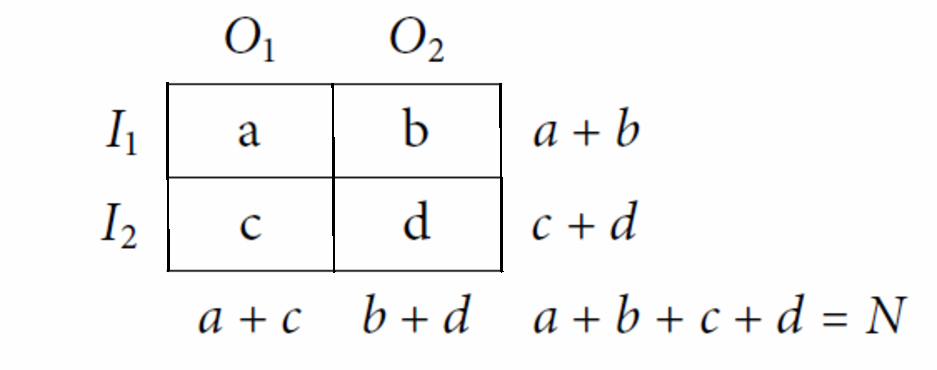
\includegraphics[width=10cm]{contingencytable}
\caption{\textsf{$2 \times 2$ contingency matrix representing the joint frequencies of two binary input ($I$) and output ($O$) variables over $N$ trials, along with row and column sums.}\label{fig:contingency}}
\end{center}
\end{figure}

The letters inside the table represent the joint frequency of the corresponding input and output occurring together.  Thus, the number of times the button is pushed and the light comes on would be represented by $a$, similarly, the number of times the button is not pushed and the light does not come on is represented by $d$.  Using the frequencies in figure \ref{fig:contingency}, the normative measure of the contingency between $I$ and $O$ can be measured by $\Delta P$:

\begin{equation}
\Delta P = P(O_1|I_1) - P(O_1|I_2) = a/(a+b) - c/(c+d)
\end{equation}

\deltap \xspace measures the difference in observed probabilities between the probabilities of success when the button is and is not pushed. In the event-onset paradigm for the illusion of control, Alloy and Abramson (1979) established \deltap \xspace as the normative standard for control.\footnote{While Jenkins and Ward (1965) used \deltap \xspace earlier, they did not use it explicitly as a measure of the illusion of control.}  Implicit in the use of this measure is the equivalence between the contingency of two variables and participant's control.  

This assumption entails a normative model for the process of estimating control in situations with a dichotomous input and output:
First, estimate the probability of success when using the input, $P(O_1|I_1)$, and the probability of success when not using the input, $P(O_1|I_2)$ through the use of frequency counts. Second, subtract the probability of success when not using the input from the probability of success when using the input.  This difference is $\Delta P$---the amount of control possessed in this situation.

Other methods of measuring contingency are either extremely similar to \deltap \xspace, such as the $\phi$ coefficient (Alloy and Abramson, 1979; Allan, 1983) or equivalent to it, such as the Rescorla-Wagner model, which reduces to the $\Delta P$ when there is only one binary input variable (Rescorla and Wagner, 1972; Danks, 2003; Glymour, 2001).

As simple as this model is, previous research has not measured participants' intermediate calculations of the probability of success and compared these values to participants' estimates of control.  Nor has previous work examined exactly what data participants observe and if their estimates are reasonable given their observations.  For example, Thompson et al. (2007), instead of recording the number of successes each participant observed, estimated the number of times that participants saw a success when pressing a button by multiplying the number of times they pressed the button by the percentage chance of a success when the button was pressed. They did not ask participants to give an estimate of this percentage, which would have been useful in determining if errors in estimates are due to inaccurate recollections of observations or an error in calculation.  While the studies in chapter \ref{chap:ioc} asked participants to estimate these percentages, they only compared the estimated $P(O_1|I_1)$ to its experimental value, not the actual observed value nor did they compare $P(O_1|I_2)$ or participants' estimated $\Delta P$ to the actual $\Delta P$.  These issues are addressed by the study in chapter \ref{chap:bioc}.

Comparing participants' estimated $P(O_1|I_1)$ and $P(O_1|I_2)$ to the actual probabilities allows us to measure how well calibrated participants are and allows us to calculate their estimated $\Delta P$.  This $\Delta P$ can be compared to both the actual control as well as the value of control that participants give.  If this $\Delta P$ differs significantly from participant's own estimate of control but is close to the actual $\Delta P$, then it is possible that the participant's definition of control is different from the experimenter's definition.  

\section{The role of prior beliefs in estimating contingencies}

Study 2 in chapter \ref{chap:ioc} asked participants to estimate the probability of success of pushing a button before starting the experiment and found that across all conditions, the mean estimate was about 45\%.  Would and should these participants allow these prior beliefs to affect their final estimates?  Alloy and Tabachnik's (1984) review of covariation research concluded that prior beliefs did indeed influence covariation assessment, furthermore, they concluded that while the use of prior beliefs was normative, in order to be `rational', one would have to discard these beliefs and make an estimate only on the observed data.  While Alloy and Tabachnik's distinction between what is normative and rational might seem odd, this dichotomy might be rephrased as a lack of congruence between the normative processes and normative outcomes expected in covariation and contingency estimation.  The normative outcome is expected to be a statistical frequentist's response: the probability of the data that has been observed. This assumption underlies the use of T-tests and ANOVA's when comparing participants' estimates with the experimentally set value.  However, if we acknowledge, as Alloy and Tabachnik did, that using prior beliefs in making our estimates is a normative process, then it is reasonable to question if they do conflict, if so, how should this be resolved? A possible solution is the use of Bayesian inference which is essentially a 'mixture' of prior beliefs and current observations. Chapter \ref{chap:model} addresses this question and a Bayesian solution in more detail.

%\section{Philosophical Assumptions with the Control}
%
%Jenkins and Ward (1965) justified asking participants to estimate their \emph{control} because ``in the context of the task it seemed to be the most natural way to communicate the technical meaning of contingency with everyday language.'' Subsequent work, such as Alloy and Abramson (1979) and Thompson et al. (2004, 2007) implicitly adopted the Jenkins and Ward's conflation of control with contingency.\footnote{Alloy and Abramson (1979) expand on Jenkins and Ward's justification by explaining that ``The relation between such events is best construed as one of controllability...Thus, control is best defined as the dependence of an outcome on a response.''} However, \emph{control} is not the first concept to be defined by correlation or contingency.  David Hume set forth his  
%  
%Underlying the use of \deltap \xspace as a measure of control is the 


\chapter{Keeping the Illusion of Control under Control}
\label{chap:ioc}

\epigraph{\SingleSpacing Appearances do indeed present cases from which a rule can be obtained according to which something usually happens, but they never prove the sequence to be necessary.}{\textit{Critique of Pure Reason}\\ \textsc{Immanuel Kant}}

\section{Introduction}
While prior research has focused on people's estimates of control over heavily chance-determined events, less research has examined people's assessments of control in situations where actual control is high. These situations are quite common in organizations and broader society more generally, and they often involve high-stake consequences--such as stopping a car by stepping on the brake, working hard to increase one's odds of being promoted, or exercising in order to lose weight. Are people's estimates of their control accurate in these situations?\footnote{This chapter, as well as parts of chapters \ref{chap:intro} and \ref{chap:history} was previously published as Gino, Sharek and Moore, 2011}  

In this chapter, we suggest these estimates are not accurate. We extend the literature on personal control and co-variation assessment by exploring people's perceptions of control across a full range of situations. We consider both heavily chance-determined situations where actual control is low (as in prior studies on the illusion of control and co-variation assessment), and situations characterized by high levels of actual control. Across three laboratory studies, we examine the psychological factors that may alter the relationship between actual control and perceived control. We propose a simple theoretical framework that can be used to study people's perceptions of control by suggesting that people have an imperfect sense of how much they control probabilistic events. Specifically, when they have very little control, we expect them to overestimate it, as demonstrated in prior work. But when they have high levels of control, we expect them to underestimate it, consistent with a case of imperfect calibration. Indeed, if people systematically overestimate their control when they have objectively little because they are unsure about how much control they have, then it is to be expected that they will systematically underestimate their control when they actually have a great deal of control. 

\section{Miscalibration in Judgment}
Are people's perceptions of ability or performance accurate? Several studies have found that perceptions of ability and performance are poorly correlated with actual performance and therefore are regressive with respect to actual performance (e.g., Burson, Larrick, \& Klayman, 2006; Moore \& Healy, 2008). Research on overconfidence has suggested that there are several sources of unsystematic error in subjective confidence that influence decision makers' judgments, ranging from misleading prior experiences (Juslin, 1994; Soll, 1996) to relying on information associated with deceptive feelings of confidence (Erev, Wallsten, \& Budescu, 1994; Heath \& Tversky, 1991; Simmons \& Nelson, 2006). 

Related research has found regressive effects in comparative judgements (Moore \& Small, 2007), as well as in judgements of accuracy (Dawes \& Mumford, 1996). When people compare themselves with others, their imperfect knowledge of others inserts an additional source of error (Krueger, 2000; Krueger \& Clement, 1997; Krueger, Acevedo, \& Robbins, 2005; McFarland \& Miller, 1990). Consequently, the worst performers overestimate their percentile ranks, whereas the highest performers underestimate theirs (Krueger \& Mueller, 2002; Kruger \& Dunning, 1999). Building on this research, Larrick, Burson, and Soll (2007) argued that some factors influence perceptions of ability and performance without influencing actual performance. For instance, certain manipulations of task difficulty may move perceptions more than actual performance.

\section{Theoretical Model and Research Hypotheses}
As this body of work demonstrates, the result of errors in judgements of perceived and actual performance is that people overestimate low performances and underestimate high performances. We argue that the same type of mis-calibration occurs in judgements of personal control because factors that influence actual control and factors that influence perceived control can move separately. Consequently, we expect people to systematically overestimate their control when they have objectively little or no control and to systematically underestimate it when they have objectively high control.

Figure \ref{fig:ioc-fig-1} illustrates the hypothetical pattern of results. As the figure shows, we expect people to have imperfect knowledge of their own control and to make regressive estimates. We also expect the linear and regressive relationship between perceived and actual control to break down as one approaches 100\% actual control. Unlike the 0\% control condition, in which random influences can create uncertainty about how much control one has, no such ambiguity is possible when one has perfect control, creating a structural asymmetry between conditions of no control and complete control. This non-linearity qualifies the proposed regression account. We should note that a similar non-linearity is expected in cases in which actual control is zero and decision makers have no way to influence the outcome (e.g., a button is not present in a task where pressing a button produces a desired outcome). That is, we expect people to be cognizant enough to realize that if there is no button present at the crosswalk, they could not have had any control over the walk signal (Matute, 1996; Shanks \& Dickinson, 1987; Wasserman, 1990).  

\begin{figure}[t]
\begin{center}
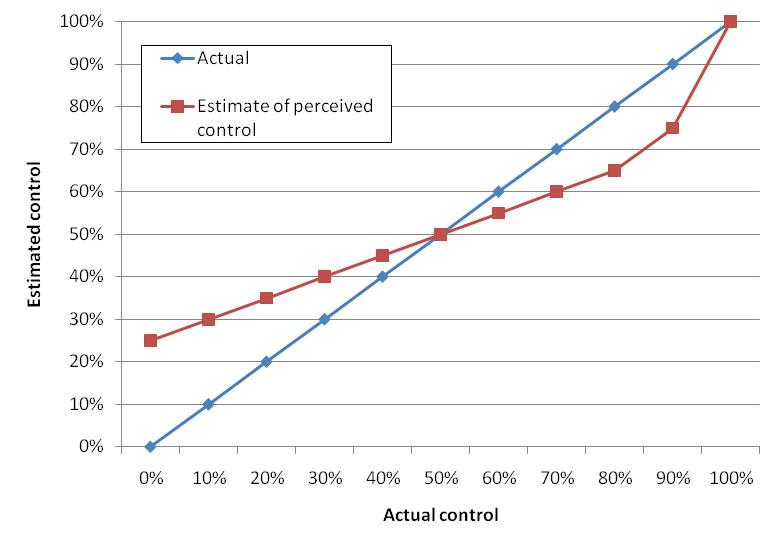
\includegraphics[width=10cm]{ioc-fig-1}
\caption{\textsf{Hypothetical Results: Estimates of perceived control as a function of actual control.}\label{fig:ioc-fig-1}}
\end{center}
\end{figure}

We find support for our main hypothesis across three laboratory studies that employ common illusion-of-control paradigms. The current research focuses on two cells that have not been compared directly by most prior research on illusory control: Nondepressives on both uncontrollable and controllable tasks. Across the three studies, our results question the conclusion that nondepressives systematically overestimate their control--a conclusion that, to date, remains widely accepted in social psychology, organizational behaviour, and behavioural decision research.

\subsection{Experimental Design Advantages}
We use experimental designs that are similar to the event-onset paradigm described in chapter \ref{chap:history}, but we introduce the measures of control used in each paradigm. Thus, in our studies we examine perceptions of control by giving participants feedback on their actions (e.g., pressing a button), by using tasks including multiple rounds, and by measuring control with questions about predictions of control and past behavior. 

Importantly, we study people's perceptions of control across a full range of situations, from situations where actual control is zero or low to situations where actual control is high or complete. In this way, our studies introduce an experimental condition that is missing from most research on the illusion of control and co-variation assessment: an objectively high-control condition.

\section{Study 1: Poor Calibration in Predicting One's Control}
Our first study examined how individuals' subjective sense of control is affected by their actual degree of control. Our main goal in this study was a critical test of the claim that people overestimate their control. Our study contributes to research on this topic by including a high-control condition.

\subsection{Method}
\subsubsection{Participants}
Participants were 80 undergraduates at a northeastern university in the United States (Mage = 21, SD = 2.03; 31\% female) who participated in exchange for course credit in their introductory business courses. 

\subsubsection{Design and procedure}
The study was described to participants as an experiment on attention and visual perception. Participants performed a vigilance task on computers. Specifically, their task was to examine a series of computer screens filled with random sequences of letters and to find instances of two same consecutive letters (e.g., ``e e'' in the sequence ``r t e e f c'') and click on them. Ten different screens were displayed, each for 90 seconds. Each of these ten rounds was divided into 18 five-second intervals. Each five-second interval began with black letters presented on a white background. We then introduced an annoyance that made it more difficult for participants to complete the task: The background went black and the letters changed from white to violet, making them more difficult to read. This change occurred at a randomly determined point during the first three seconds of the five-second interval. In addition, there was a button on the screen that read ``STAY WHITE''. If the button worked when participants pressed it, then the screen would remain white with black letters for the remainder of the five-second interval. Participants could press the ``STAY WHITE'' button only once within each five-second interval. Participants learned all of this information in the experimental instructions (reported in Appendix \ref{app:study-1-instructions}. Note that in this task, finding correct instances of two same consecutive letters did not have any impact on whether the background changed color, but pressing the ``STAY WHITE'' button did.

In fact, pressing the ``STAY WHITE'' button kept the screen white with a certain probability p, where p varied across conditions. We manipulated participants' actual level of control by varying the value of p. There were four conditions in the experiment: high control (p = 85\%), medium control (p = 50\%), low control (p = 15\%), and no control (p = 0\%). We predicted that people would overestimate their control only in the low- and no-control conditions. 

After completing the task, participants were asked the following questions, which were designed to assess their perceived control: (1) ``How much control do you think you had when trying to stop the page-color switching? (1 = no control at all; 7 = complete control)''; (2) ``How often do you think pressing the ``STAY WHITE'' button produced the desired outcome (keep the page white with black text)?  Please indicate what percentage of the time pressing the button worked. (0 = never; 100 = always)'' 

\subsection{Results}
\subsubsection{Task performance}
We first examine the number of correct pairs participants were able to identify and the total number of times they clicked on the page to identify instances of two same consecutive letters. There were no significant differences in total number of instances participants correctly identified across conditions, $F(3, 76) < 1, p = .50, \eta^2 = .03$. Similarly, there were no significant differences across conditions in ``false alarms'' or incorrectly identified instances of two same consecutive letters $(F(3, 76) < 1, p = .42, \eta^2 = .04)$.

\subsubsection{Perceived control}
As predicted, people overestimated their control in the low-control condition (24\% versus the real probability equal to 15\%), $t(19) = 6.04, p < .001$, and underestimated it in the high-control condition (39\% versus the real probability equal to 85\%), $t(19) = -7.77, p < .001$. These results are consistent with our main hypothesis and suggest that people systematically overestimate their control when it is objectively low and systematically underestimate it when it is objectively high. These results are summarized in Table \ref{tab:ioc-1} and depicted graphically in Figure \ref{fig:ioc-fig-2}.

\begin{table} 	
	\setlength{\extrarowheight}{4pt}
	\begin{tabulary}{\linewidth}{cCCC}
	\toprule
	Condition & Actual button efficacy & Perceived button efficacy: How often do you think the button worked? (0-100) & Perceived Control: How much control do you think you had? (1-7)\\
	\midrule
	High   & 85\% & 39.00\%$_a$ (21.95) & 2.75$_a$ (1.55) \\ 
	Medium & 50\% & 36.11\%$_a$ (20.32) & 2.60$_a$ (1.00) \\
	Low    & 15\% & 24.05\%$_b$ (17.70) & 1.65$_b$ (0.59) \\
	Zero   & 0\%  & 25.01\%$_b$ (18.19) & 1.45$_b$ (0.51) \\
	\bottomrule	 	
	\end{tabulary}
	\caption{Responses to post-task questionnaire, by condition, Study 1. Standard deviations appear in parentheses. Figures in the same column with different subscripts are significantly different from one another.\label{tab:ioc-1}}
\end{table}

\begin{figure}[t]
\begin{center}
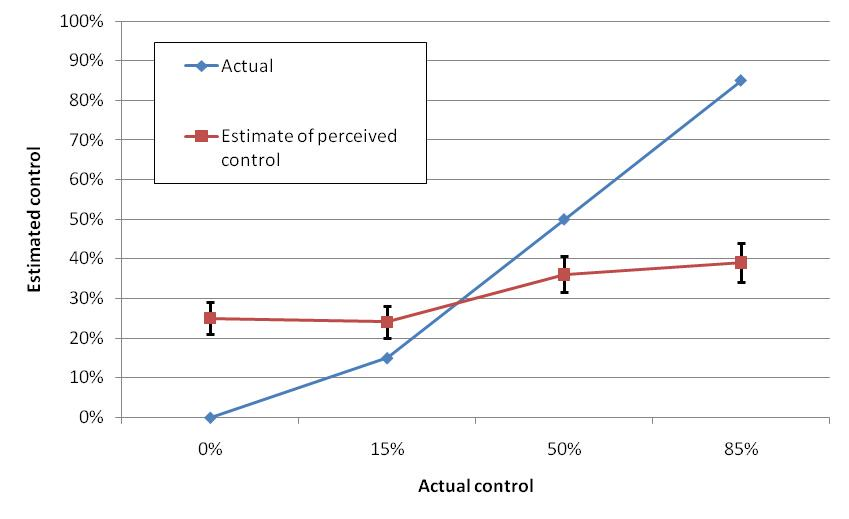
\includegraphics[width=10cm]{ioc-fig-2}
\caption{\textsf{Participants' estimates of perceived control as a function of actual control, Study 1. Error bars show standard errors.}\label{fig:ioc-fig-2}}
\end{center}
\end{figure}

The study included a second measure of perceived control, which consisted of a self-reported rating. As Table 1 shows, participants reported having more control in the high-control condition than in both the low-control condition, $t(38) = 2.97, p = .005$, and in the no-control condition, $t(38) = 3.56, p = .001$. These results suggest that participants realized there were differences in control across conditions, as reflected in their judgements of perceived control. Nonetheless, their estimates were regressive.

\subsection{Discussion}
The results of Study 1 support the hypothesis that people systematically overestimate their control when they have low control and underestimate it when they have high control. These findings are inconsistent with the claim that people generally overestimate how much control they have (Taylor \& Brown, 1988). However, we should note that our findings are not at odds with the empirical results from research on illusion of control, which has documented many important influences on people's subjective sense of control. Indeed, illusion-of-control studies rarely ask people directly to estimate their level of control (e.g., Langer, 1975; Langer \& Roth, 1975). Instead, they include other measures, such as betting choices or predictions of future success, but do not directly elicit beliefs about individuals' perceived control using measures whose accuracy can be objectively assessed (Abramson \& Alloy, 1980). 

In Study 1, participants' estimates of button effectiveness when the button worked (i.e., in the high-control condition) were quite low. We believe this was due to the properties of the task employed in the study. By asking participants to focus on the goal of finding two same consecutive letters, they may have not pressed the ``STAY WHITE'' button as frequently as we expected, and thus they may not have exploited the opportunity to learn about how often the button worked in producing the desired outcome. Indeed, on average, the ``STAY WHITE'' button was pressed 78 times (SD = 60.30) across conditions out of a possible 180 times. In addition, the annoyance we used may not have been successful in making it more difficult for participants to complete the task. We address these potential limitations in Study 2.

\section{Study 2: Examining Situations of Complete Control}
The goal of our second study was twofold. First, we wanted to replicate the same findings of Study 1 using a modified task that addresses the limitations noted above. Second, we extended the number of conditions considered when manipulating actual control and included a condition in which actual control was 100\%.

\subsection{Method}
\subsubsection{Participants}
Two-hundred twenty undergraduates at a large southeastern university in the United States ($M_{age} = 21, SD = 2.18; 51\%$ female) participated in exchange for \$7. Participants also had the opportunity to earn an additional \$5 depending on their performance on the task.	
Design and procedure. Our second study employed the same task and procedure of Study 1, with four differences. First, we lowered the brightness of each computer monitor in the lab room to make the annoyance used in the task more effective. Second, we introduced an incentive for participants, promising an additional \$5 to those who correctly found more than 90\% of the two consecutive same letter instances. Third, after participants read the initial instructions to the task and before they engaged in it, we asked them to guess the percentage of the time pressing the button would keep the screen white (0 = never; 100 = always). Finally, we considered a larger number of conditions for our manipulation of actual control. Specifically, we included seven levels of actual control: complete (100\%), high (90\%), medium-high (75\%), medium (50\%), medium-low (25\%), low (10\%), and no control (0\%).

\subsection{Results}

\subsubsection{Task performance}
As in Study 1, we did not find significant differences in the total number of instances participants correctly identified across conditions, nor in the total number of instances participants identified incorrectly (both Fs < 1).

\subsubsection{Initial predictions}
We first examined the initial predictions participants made regarding the percentage of the time pressing the ``STAY WHITE'' button would keep the screen white. Such predictions did not differ across conditions (F < 1). As shown in Table \ref{tab:ioc-2}, on average participants predicted the button would work almost 45\% of the time. 

\subsubsection{Estimates of control}
The mean values for our measures of perceived control are reported in Table \ref{tab:ioc-2} and depicted graphically in Figure \ref{fig:ioc-fig-3}. Replicating the results of Study 1, people overestimated their control in the no-control condition (22\% versus the real probability equal to 0\%, 95\% confidence interval of the difference=[17.49, 25.74]), in the low-control condition (26\% versus the real probability equal to 10\%, t[30] = 5.04, p < .001), and in the medium-low condition (34\% versus the real probability equal to 25\%, t[31] = 2.19, p < .04). At the same time, they underestimated their control in the high-control condition (73\% versus the real probability equal to 90\%, t[30] = -10.91, p < .001) and in the medium-high control condition (56\% versus the real probability equal to 75\%, t[31] = -8.87, p < .001). Interestingly, in the medium-control condition, participants still underestimated their level of control (42\% versus the real probability equal to 50\%, t[31] = -2.76, p = .01). In the complete-control condition, all participants except for one indicated that the button worked 100\% of the time. This result is consistent with our proposed model for people's perceptions of control (see Figure \ref{fig:ioc-fig-1}). 

\begin{table} 	
	\setlength{\extrarowheight}{4pt}
	\begin{tabulary}{\linewidth}{lLLLL}
	\toprule
	Condition & \mbox{Actual} \mbox{button} \mbox{efficacy} & Predicted button efficacy: How often do you think the button will work? (0-100) & Perceived button efficacy: How often do you think the button worked? (0-100) & Perceived Control: How much control do you think you had? (1-7)\\
	\midrule
	Complete      & 100\% & 41.52\% (15.60) & 99.94\%$_a$ (0.36)  & 6.81$_a$ (0.40)\\ 
	High          & 90\%  & 46.61\% (20.44) & 72.52\%$_a$ (8.93)  & 5.26$_a$ (1.03)\\ 
	Medium-High   & 75\%  & 44.38\% (21.93) & 56.22\%$_b$ (11.98) & 4.00$_a$ (1.19)\\ 
	Medium        & 50\%  & 45.06\% (21.83) & 42.34\%$_a$ (15.68) & 2.88$_a$ (1.10)\\
	Medium-Low    & 25\%  & 48.62\% (21.26) & 33.91\%$_b$ (23.06) & 2.16$_b$ (1.30)\\ 
	Low           & 10\%  & 41.68\% (21.38) & 25.55\%$_b$ (17.19) & 1.71$_b$ (1.37)\\
	Zero          & 0\%   & 44.94\% (23.73) & 21.61\%$_b$ (11.25) & 1.29$_b$ (0.46)\\
	\bottomrule	 	
	\end{tabulary}
	\caption{Responses to post-task questionnaire, by condition, Study 2. Standard deviations appear in parentheses. Figures in the same column with different subscripts are significantly different from one another.\label{tab:ioc-2}}
\end{table}

\begin{figure}[t]
\begin{center}
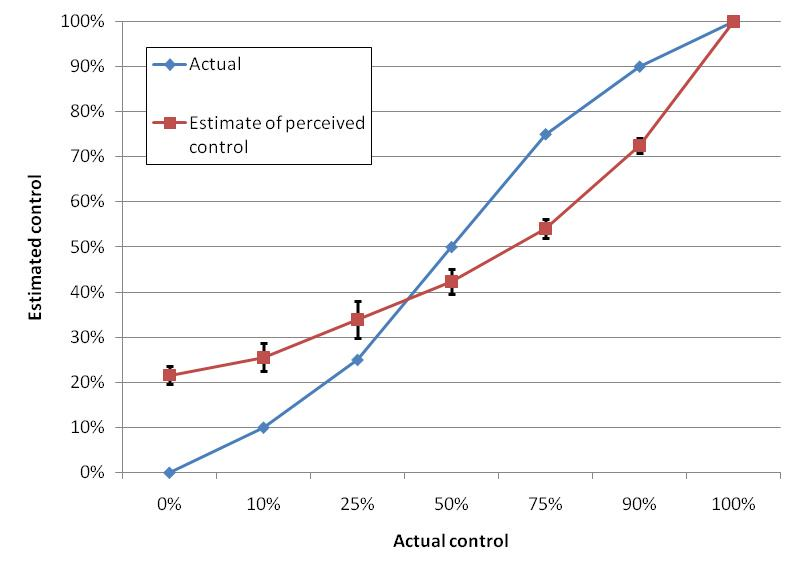
\includegraphics[width=10cm]{ioc-fig-3}
\caption{\textsf{Participants' estimates of perceived control as a function of actual control, Study 2. Error bars show standard errors.}\label{fig:ioc-fig-3}}
\end{center}
\end{figure}


Study 2 also included the second measure of perceived control used in Study 1. As Table \ref{tab:ioc-2} shows, the results for the self-reported measure of perceived control are consistent with participants' estimates of button efficacy. Participants' ratings of perceived control suggest that they realized there were differences in control across conditions. Nonetheless, their estimates were regressive.

\subsection{Discussion}
The results of Study 2 provide further support for our main hypothesis. We find two opposite errors that occur at the floor and the ceiling of actual control: people overestimate their control when they have low control and underestimate it when they have high control. Consistent with our proposed model, the linear and regressive relationship between perceived and actual control broke down as the level of actual control approached 100\%. At a 90\% level of actual control, we still observed underestimation of perceived control, but when actual control was complete (100\% actual control condition), participants' estimates of control were accurate.

When describing our proposed model, we suggested that another condition under which the model would break down is the one in which actual control is zero and there is no opportunity for participants to influence the desired outcome. We conducted a study on a non-overlapping group of participants from the same population as in Study 1 (N = 32) and presented them with the same task used in Study 2. However, this time there was no ``STAY WHITE'' button they could press. As one would expect, when asked to estimate their control over the action producing the desired outcome (page color-switching), all participants indicated they had no control.


\section{Study 3: Motivation and Illusion of Control}
As we have noted, almost all the past research on illusory control has employed tasks in which participants had little or no actual control. Yet one of the more important studies in the literature on perceived control actually did include a high-control condition: Alloy and Abramson's (1979) first experiment. The authors used a paradigm in which participants were presented with a series of events--e.g., a green light that either came on or not over a series of rounds--and were asked to estimate how much they could control the appearance of the light by pressing a button. Participants had to decide whether or not to press the button and then observed whether the light came on. In the high-control condition, the light came on with 75\% probability when a participant pushed the button and never came on when the participant didn't push it. Alloy and Abramson's (1979) first experiment also included a no-control condition and a moderate-control condition in which the light appeared with 0\% or 25\% probability, respectively, when a participant pushed the button. 

\subsection{Measuring Perceived Control}
Our third study employed Alloy and Abramson's (1979) popular ``button-light'' paradigm. However, we used a less controversial measure of perceived control. In Study 3, we asked participants to estimate both the probability the light would come on when they pressed the button and when they did not press the button. One benefit of this approach is that it allows us to ``unconfound'' the extremes of control with the extremes of the response scale. For example, if both pressing and not pressing the button produce the desired outcome (in our study, the appearance of a blue circle on a computer screen) with 50\% probability, then pushing the button exerts no control over the outcome. However, it is still possible to underestimate the efficacy of button-pushing by reporting that the button comes on less than 50\% of the time following a button-push. For Alloy and Abramson's difference measure, \deltap, by contrast, this situation represents zero control, and the only possible error participants could make would be to overestimate control. Thus, our third study includes measures related to estimates of contingency between one's responses and outcomes as well as estimates of perceived control.
In addition to employing better measures of perceived control than those used in prior research, our study also allows us to assess Thompson's control heuristic (discussed in chapter \ref{chap:history}). While Thompson et al. (2004) tested the control heuristic, they only examined non-contingent situations where participants had zero control (as measure by \deltap). Thus, their study leaves unanswered the question of how well the control heuristic explains people's perceptions of control when actual control is greater than zero. In our third study, we used a manipulation of motivation similar to that used by Thompson et al. (2004, 2007). We tested whether their results generalize to a circumstance in which people actually have some control.   

\subsection{Method}

\subsubsection{Participants}
One hundred and two college students at a large southeastern university in the United States (Mage = 21, SD = 1.83; 53\% female) participated in the study for pay. On average, participants received \$10 for their participation in the study (including a \$3 show-up fee). 

\subsubsection{Design and procedure}
The experiment employed a 2 (actual control: high control vs. low control) x 2 (motivation: pay vs. no-pay) between-subjects design. Upon arriving at the laboratory, participants were seated at computers and were randomly assigned to one of the four experimental conditions. 

Participants were presented with one of two contingency problems, which differed in their degree of contingency or control. The procedure and 
instructions for each of the two contingency-problem groups were identical. Participants could make one of two possible responses (using a computer mouse to press or not press a button shown on the screen) and receive one of two possible outcomes (the appearance of a blue circle or no blue circle). As in Alloy and Abramson's (1979) study, all participants were told that in this problem-solving experiment, their task was to learn what degree of control they had over whether or not a blue circle appeared on the screen and that they had the option of pressing or not pressing the button in each trial. In addition, participants in the pay condition were told that they would receive \$.20 every time the blue circle appeared on the screen during the 40 trials, for a maximum possible payment of \$8. 

More specifically, for each round, after the word ``START'' appeared on the screen, participants had the option of pressing a button. If they wanted to press the button on a given round, they had to press it within two seconds after the word ``START'' appeared. In the last second of each three-second trial, after participants had pressed the button (or not), a blue circle sometimes appeared on the screen. Its appearance depended on their response and on the contingency problem to which they had been assigned. The interval between trials lasted half a second.  

Before the experiment started, participants learned that there were four possibilities for any given round: ``1) you press and the blue circle does appear; 2) you press and the blue circle does not appear; 3) you don't press and the blue circle does appear; 4) you don't press and the blue circle does not appear.'' Participants also read, ``You will play 40 rounds. After the 40 rounds, you will be asked to indicate how much control you think you had over the appearance of the blue circle. It may turn out that you will have no control, that is, your responses will not affect the appearing of the blue circle, or it may turn out that you will have some degree of control, either complete or intermediate, that is, one response produces the appearing of the blue circle more often than does the other.''

After completing 40 trials, participants answered a series of questions that appeared in a different randomly determined order for each participant. Specifically, we asked participants to (1) ``rate the degree of control your actions (pressing and not pressing the button) exerted over the outcome (appearance of the blue circle)'' using a percentage between 0 and 100\%. This question replicates the way that Alloy and Abramson (1979) and Thompson et al. (2007) elicited perceptions of control. In addition, we asked participants: (2) ``Please estimate the percentage of rounds on which the blue circle appeared regardless of which response you made,'' (3) ``Please estimate the percentage of rounds on which the blue circle appeared when you pressed,'' and (4) ``Please estimate the percentage of rounds on which the blue circle appeared when you did not press.''

We manipulated control by varying the rate at which the two possible actions (pushing or not pushing the button) produced a blue circle on the screen. In the high-control condition, one action produced the blue circle 90\% of the time, whereas the other one produced the blue circle 10\% of the time. In this condition, actual control was 80\%, according to Alloy and Abramson's (1979) difference measure. In the low-control condition, one action produced the blue circle 60\% of the time, whereas the other action produced the blue circle 40\% of the time. In this condition, actual control equaled 20\%, according to Alloy and Abramson. We counterbalanced whether pressing or not pressing the button was more likely to produce the blue circle in order to rule out the possibility that attributions of control would be biased by a natural tendency to associate action (pushing the button) with producing a consequence. 

\subsection{Results}

\subsubsection{Button-pressing}
On average, people pressed the button in 23 of the 40 rounds. Our manipulations affected button-pressing, as revealed by a 2 (control) $\times$ 2 (action: press vs. no-press) $\times$ 2 (motivation) ANOVA. Participants pressed the button more often when pressing improved their chances of getting the blue circle (M = 27.96, SD = 9.78) than when it did not $(M = 17.50, SD = 11.23), F (1, 94) = 30.52, p < .001, \eta^2 = .25$. The motivation $\times$ action interaction emerged as highly significant, $F(1, 94) = 15.40, p < .001, \eta^2 = .14$, since payment led the action manipulation to have a strong effect. This is because when participants knew they would be paid for getting a blue circle, they pressed the button a great deal when pressing improved their chances of getting the blue circle $(M = 30.62, SD = 8.38)$, and when not pressing improved their chances of getting a blue circle, they pressed much less $(M = 12.67, SD = 10.53), t(51) = 6.85, p < .001$. When they weren't being paid for getting a blue circle, the action manipulation did not have a significant effect on participants' overall rate of button-pushing $(M = 25.08, SD = 10.53 vs. M = 22.72, SD = 9.65), t(47) < 1, p = .42$. Finally, the control $\times$ action interaction was also significant, $F(1, 94) = 15.25, p < .001, \eta^2 = .14$. When participants had high control, they pressed the button more often when pressing improved their chances of getting the blue circle $(M = 29.81, SD = 8.51)$ than when it did not $(M = 11.69, SD = 9.61), t(50) = 7.20, p < .001$. But when participants had low control, they did not differ in their button-pushing behavior $(M = 25.96, SD = 10.82 vs. M = 23.31, SD = 9.73), t(48) < 1, p = .37$.

\subsubsection{Perceptions of control}
The first question on the post-task questionnaire asked participants to rate their level of control over the outcome. We submitted their answers to a 2 (control) X 2 (action: press vs. no-press) X 2 (motivation) ANOVA. The results revealed a main effect for control: Those in the high-control condition estimated they had 64\% control (SD = 26.75), whereas those in the low-control condition estimated they had 30\% control $(SD = 17.42), F (1, 94) = 55.21, p < .001, \eta^2 = .37$. The main effect for motivation was also significant, $F(1, 94) = 5.64, p = .02, \eta^2 = .06$: participants with a monetary incentive estimated their level of control as higher $(M = 53.57, SD = 23.54)$ than did those in the no-pay condition $(M = 40.41, SD = 30.97)$. This result is consistent with the ``control heuristic'' theory of Thompson and her colleagues, which suggests that the motivation to exert control leads to increases in perceived control. We found no other significant effect in this analysis. 

\subsubsection{Estimates of contingency}
Our concerns regarding the correct interpretation of this first vague question led us to include more specific questions. We asked our participants to estimate (a) the percentage of the time the blue circle appeared on the screen after they pressed the button and (b) the percentage of time the blue circle appeared when they did not push the button. Based on these two questions, we created a measure for perceived success of the efficacious action (either pressing or not pressing the button). This measure was equal to participants' answer to either question (a) or (b), depending on whether they were in the condition in which pressing (or not pressing) the button was more likely to produce the blue circle. This measure allows us to determine whether participants over- or underestimated control. Participants' responses do not appear to show overestimates of control. In the high-control condition, efficacious action produced the blue circle with 90\% probability, and participants estimated that it worked 60\% of the time (SD = 33.68). 
A one-sample t-test shows that this figure is significantly below the actual value of 90\%, t(51) = -6.37, p < .001. 

In the low-control condition, the efficacious action was followed by the blue circle 60\% of the time, but participants estimated that the action worked only 41\% of the time (SD = 18.17). This is a significant underestimate, $t(50) = -7.30, p < .001$. Our paradigm made it possible even for those in the low-control condition to underestimate their level of control, and they did.

A 2 (control) $\times$ 2 (motivation) ANOVA revealed that the perceived success rate of the efficacious action was influenced by our manipulation of control $( F[1, 98] = 11.49, p = .001, \eta^2 = .11)$ and by motivation $( F[1, 98] = 4.00, p < .05, \eta^2 = .04)$ in the expected direction. The control $\times$ motivation interaction was insignificant. These results are summarized in Table \ref{tab:ioc-3}. The presence of an effect for motivation is consistent with the ``control heuristic'' posited by Thompson and her colleagues (1998, 2004, 2007).  

\begin{table} 	
	\setlength{\extrarowheight}{4pt}
	\begin{tabulary}{\linewidth}{lLLL}
	\toprule
	Level of Control & Motivation & Actual success rate & Estimated success rate \\
	\midrule
	Complete      & Pay    & 90\% & 64.83\%$_a$ (29.83) \\ 
	              & No Pay & 90\% & 54.43\%$_a$ (37.87) \\ 
	Low           & Pay    & 60\% & 47.00\%$_b$ (16.68) \\ 
	              & No Pay & 60\% & 35.96\%$_c$ (18.17) \\
	\bottomrule	 	
	\end{tabulary}
	\caption{Participants' perceived estimated success of the efficacious action by condition, Study 3. Standard deviations appear in parentheses. Figures in the same column with different subscripts are significantly different from one another.\label{tab:ioc-3}}
\end{table}

\subsubsection{Additional analyses}
We conducted further analyses to test the influence of pressing the button on perceptions of control as measured by participants' perceived success of the efficacious action. We hypothesized that such button pressing would moderate the relationship between actual control and perceived control, such that actual control would be associated with perceived control only when participants had engaged in enough trials to gather information about the outcomes of their actions. We tested this hypothesis using the moderated regression procedures recommended by Aiken and West (1991). We standardized the button-pressing behavior variable and then multiplied it by the actual control variable to create an interaction term. In our regression analyses, we controlled for the motivation manipulation and its interactions with actual control. The results of our regression analyses are displayed in Table \ref{tab:ioc-4}. We found a significant interaction between actual control and button pressing. To interpret the form of this interaction, we plotted the simple slopes for the relationship between actual control and perceived control at one standard deviation above and below the mean of button pressing (see Figure \ref{fig:ioc-fig-4}). When participants pressed the button rarely, actual control was not associated with perceived control ($\beta$ = .16, p = .20). When participants pressed frequently, the simple slopes indicated that actual control was associated with perceived control ($\beta$ = .61, p < .001). Thus, the number of times participants pressed the button moderated the relationship between actual control and perceived estimated success of the blue-circle-producing action. 

\begin{table} 	
	\setlength{\extrarowheight}{4pt}
	\begin{tabulary}{\linewidth}{LLL}
	\toprule
	              & Model 1 & Model 2 \\
	\midrule
	Controls & & \\
	\quad Age           & .10 & .08 \\
	\quad Sex (Male=1, Female=0) & .14 & .13 \\
	Independent variables & & \\
	\quad Control (high=1,low=0) & .36*** & .33** \\
	\quad Motivation (pay=1,no pay=0) & .26** & .23 \\
	\quad Button pressing & .42*** & .15 \\
	2-way interactions & & \\
	\quad Control $\times$ Motivation & & .05 \\
	\quad Control $\times$ Button pressing & & .33* \\
	$R^2$ & .34 & .38 \\
	Overall $R^2$ & .58 & .62 \\
	F(5,96) & 9.82*** & 8.21*** \\	
	\bottomrule	 	
	\end{tabulary}
	\caption{Hierarchical regression results on perceived estimated success of the blue-circle producing action, Study 3. The table reports standardized coefficients. \small Notes: $* p < .05, ** p < .01,*** p < .001$. When we entered the interaction terms in a separate step between the first and second model, variance explained increased by 4\% from $R^2 = .34$ to $R^2 = .38$, $F(2, 94) = 3.11, p < .05$.\label{tab:ioc-4}}
\end{table}

\begin{figure}[t]
\begin{center}
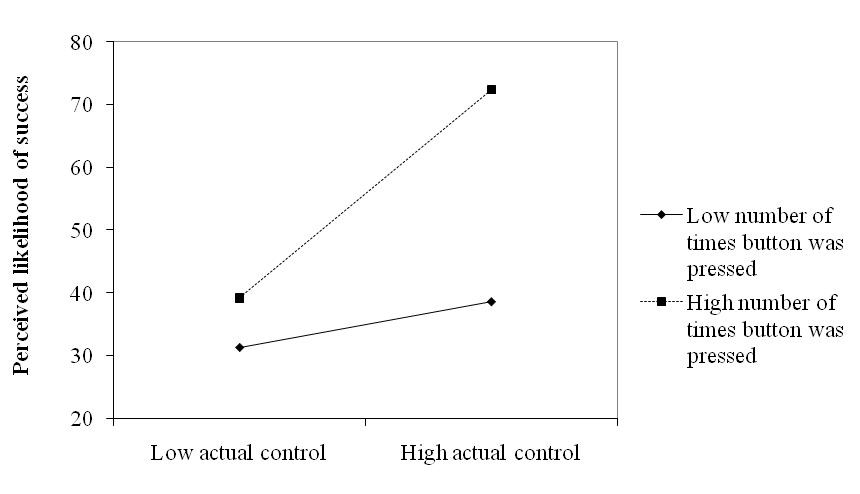
\includegraphics[width=10cm]{ioc-fig-4}
\caption{\textsf{Simple slopes for participants' perceived estimated success of the blue-circle-producing action, Study 3.}\label{fig:ioc-fig-4}}
\end{center}
\end{figure}

\subsection{Discussion} 
The results of our third study provide further support for our main hypothesis: individuals have inaccurate perceptions of control and their estimates of contingency are also miscalibrated. Our third study also casts further doubt on the conclusion that people generally overestimate how much control they have. Indeed, we observe a general underestimation of control. Consistent with the control heuristic theory proposed by Thompson and her colleagues, our third study also finds support for the role of motivation in inflating people's estimates of personal control: Participants' judgements of control were higher when they had an incentive to be effective (i.e., participants were paid when the blue circle appeared on the screen). However, even those paid for blue circles underestimated their control in the high-control condition. And the effect of motivation did not interact with the actual degree of control, suggesting that these two influences on perceived control are most appropriately modeled with these two parameters as main effects (see Krueger \& Clement, 1997). 

\section{General Discussion}
The issue of whether people overestimate their control over probabilistic events has obvious implications for a number of important domains. For instance, people who overestimate their control over others will make incorrect attributions regarding their influence over others' behavior (Morris, Sim, \& Girotto, 1998). Those who overestimate their personal control may make bad decisions about where to direct their efforts (Ajzen, 1991; Vroom, 1964), whether or not to listen to others' opinions (Gino \& Moore, 2007; Tost, Gino, \& Larrick, 2010), or about whether to enter a market or start a new business (Moore \& Cain, 2007; Moore, Oesch, \& Zietsma, 2007). Overestimates of control may make people too slow to respond to feedback that suggests their efforts are misplaced (Pearce \& Porter, 1986). On the other hand, the positive illusions literature claims that an exaggerated sense of personal control is conducive to mental health and persistence through life's many frustrations (Taylor \& Brown, 1988).  

Given the relevance of accuracy in estimation of personal control, it is probably no surprise that many scholars have studied when and why people overestimate their control. This research has found that people behave as if they think they can exert more control over avoiding accidents when they are driving (Horswill \& McKenna, 1999), over games of chance (Langer, 1975, 1977), and over the onset of a light in laboratory tasks (Alloy \& Abramson, 1979) than objective circumstances warrant. Based on this and related evidence, scholars have concluded that people suffer from an illusion of control. In the words of Russo and Shoemaker (1989, p. 173): ``People often exaggerate the extent to which they control events.'' Thompson's 2008 textbook tells us: ``The illusion of control refers to the tendency for people to believe that they exert more influence over situations than they actually do.'' And Gilbert (2006) writes, ``Our desire for control is so powerful, and the feeling of being in control is so rewarding, that people often act as though they can control the uncontrollable'' (p. 22).  

Do people systematically overestimate their control? We believe there is reason to doubt that they do. We found little evidence of systematic overestimation of control in our three studies. Indeed, the only circumstance in which our participants overestimated their control was when they had very little control and when our measure made it difficult or impossible for them to underestimate their control. We have presented a theoretical model for understanding people's perceptions of control. The model is based on a very simple assumption: It is common for people to make errors regarding how much control they have. Consequently, when control is objectively low, people tend to overestimate it. When control is objectively high, however, we expect people to underestimate it. By focusing on domains in which people have little control, prior research has created the illusory impression that overestimation of control is more frequent than it actually is. Here, we have provided what we believe is a more comprehensive account of control perceptions by examining a full range of situations where actual control vary from 0\% to 100\%.

It is also interesting to note that, contrary to prior research on the illusion of control, the grand mean of the estimates participants provided for perceived control was too low across our studies. This mean-level effect is orthogonal to our regression account, but it is important to point out, as it suggests that the general tendency of people to overestimate control may not be universal.

\subsection{Limitations}
Our model has little to say about the many moderators of perceived control that previous research has documented. For instance, Gollwitzer has shown that people are more likely to perceive control where there is none when they are in an implemental rather than a deliberative mindset (Gollwitzer \& Kinney, 1989; Heckhausen \& Gollwitzer, 1987; Taylor \& Gollwitzer, 1995).  Furthermore, it may be the case that depression and/or dysphoria are associated with reductions in perceived control (Alloy \& Abramson, 1979; Alloy, Abramson, \& Viscusi, 1981). A number of other factors also influence the tendency for people to feel they have control, including the presence of competition or skill-related performance (Thompson et al., 1998). We do not question that these factors are important, and we believe future research would benefit from examining how they interact with actual level of control to influence perceived control.

We do question, however, whether there is a general tendency to overestimate one's level of control. The results of previous studies in which participants have zero control provide weak evidence on the question, since the designs of these experiments usually make it impossible for people to underestimate control. Any error in participants' estimates of control must result in overestimates. In our third experiment, where our design makes it possible for participants in the low-control condition to underestimate their degree of control, we do in fact find that they underestimate their control. 

Our findings need to be qualified by a number of limitations that suggest directions for future research. First, across our experiments, we asked participants to estimate their level of control over the link between past actions and outcomes. As we noted earlier, the classic studies by Langer and colleagues on the illusion of control employed paradigms in which participants estimated their level of control over the link between future actions and outcomes. Thus, if we restrict the use of the label ``illusion of control'' for cases in which perceptions of control are measured by using this classic paradigm, then we still cannot draw conclusions about people's tendency to over or under-estimate their control over future actions in the presence of uncertainty based on the results of our studies. Future studies investigating individuals' perceptions of control over both future and past events characterized by different levels of objective control may further advance our understanding of people's judgments of perceived control. 

Second, in presenting our model, we did not provide details on how exactly regressive judgments might arise in illusion of control or co-variation assessment tasks. We believe that regressive judgments result from the following simple model: Observed frequency on an event (which may be close to the true frequency of the event) plus error plus prior beliefs. In this model, the error term would incorporate both psychological factors and random noise. Our studies cannot clearly demonstrate whether this type of model and errors are the ones people are using in estimating personal control. Future research could explore this model directly with the goal of identifying the weight each of the factors has in determining the degree of control people perceive they have over outcomes that are completely or partly determined by chance. Future research could also examine other mechanisms that may lead people to make regressive estimates. One such factor is uncertainty; people may be uncertain about how much control they have over outcomes. These two mechanisms, error and uncertainty, differ in an important way: while error leads to increased variance in individuals' estimates, uncertainty leads to reduced variance.  Future research investigating these mechanisms directly would deepen our understanding of how people make regressive judgments when they estimate their level of control over outcomes.

Future work on people's perceptions of control could also examine individuals' estimate at a higher level of granularity. In our studies, we compared participants' estimates of success rates by representing control to the objective level of control. In the future, studies could compare participants' estimates directly to their observations over the rounds included in the task. In addition, as we did in Study 3, future studies could employ various measures of control that include both self-reports and estimates of contingency and success. Finally, research could examine the types of heuristics people use to form their estimates of control and the factors that led them to choose one heuristic over another. These various investigations would advance our understanding of the psychology of perceived control.

\subsection{Theoretical Implications}
The results of our three studies cast doubt on the claim that people systematically overestimate their control. Our research underscores the importance of examining the complete range of actual control in the study of judgments of personal control. We suggested that a complete picture takes into account both task characteristics (e.g., the level of actual control) and different influences on perceptions (e.g., depression). Future research could investigate the role of other factors, such as task familiarity or dispositional optimism, in estimation of personal control. 

Our work contributes to decision-making research on overconfidence and better-than-average effects. This body of work has found that perceptions of ability and performance are driven powerfully by characteristics of the task (e.g., its difficulty). Here, we have demonstrated that similar errors in judgment occur when people estimate their personal control over outcomes. Our results do not suggest that people are necessarily directionally biased (to either overestimate or underestimate control), but they are nevertheless inaccurate in their estimation of personal control. Furthermore, to the best of our knowledge, our research provides the first attempt to clearly distinguish between perceptions of personal control and general regression effects in individuals' assessment of co-variation, as actual control varies from low to high levels. 

Finally, our work contributes to prior literature on personal control. Across disciplines, ranging from psychology and anthropology to sociology and organizational behavior, various scholars have examined the effects that personal control over one's work environment has on both the individual and the organization (e.g., Deci \& Ryan, 1985; Holzberg \& Giovannini, 1981; Thomas, 1989). For instance, this research has found that personal control facilitates work involvement and workplace satisfaction (see Ashforth \& Saks, 2000 for in-depth discussion). Our research suggests that perceptions of control are often inaccurate, with potentially relevant consequences for people's behavior in the workplace. Future research could investigate how organizations and their managers can successfully reduce inaccuracies in workers' perceptions of control.  

\subsection{Practical Implications}
There are a great many important situations in life over which people have very little control. Some of these situations have relevant implications for both group and organizational processes and outcomes. For instance, people might overestimate the control they have in hiring excellent employees, the success of a new product, or the chances their entrepreneurial venture will succeed. It ought not be surprising that people are eager to find ways of influencing these events and that some inevitably will adopt superstitious beliefs that overestimate their control (Matute, 1994, 1995). To a great extent, this is simply a product of the fact that it is not possible to underestimate control when one has none; any mistake in estimating control can only lead to overestimation. We are reluctant to accuse pedestrians in New York of suffering from the illusion of control if they push the ``walk'' button, as it is reasonable for them to believe that pushing the button could speed their crossing. 

There are a number of practical implications of the effects observed in our studies. When people overestimate their degree of control, they may engage in easy strategies to achieve a particular outcome and avoid the more difficult actions that may be needed. For instance, if a manager overestimates her control over the success of a merger or the launch of a new product, she may spend too little time questioning the project's viability at the outset. Similarly, if a prospective employee perceives that she has more control over her negotiated salary than is warranted, she may use ineffective strategies in the negotiation. Similar inefficiencies in the use of time, strategies, and resources may also occur when people underestimate their control. In this case, people may not exert the maximum effort required to successfully accomplish a task (e.g., working extra hours) because they underestimate their control over the outcome (e.g., obtaining a promotion). A better understanding of when judgments of personal control are likely to be inaccurate may help to educate people about the ways in which their estimates of personal control are miscalibrated.

\section{Conclusion}
Most studies of the illusion of control and co-variation assessment have used contexts or tasks in which participants had little or no control (e.g., Alloy \& Abramson, 1979; Langer, 1975; Thompson et al., 2004). This research has found that people tend to overestimate their control. In this paper, we suggest that by focusing on situations marked by low control, prior research has created the illusion that people systematically overestimate their level of control. Consistent with this previous research, we find that people overestimate their control when their actual control is low or zero. However, when their actual control is high, we find that they tend to underestimate it. These results suggest a simpler and more mundane explanation of how people judge their degree of control over desired outcomes: they inaccurately estimate their personal control. 

\chapter{Modeling the Illusion of Control}
\label{chap:model}

\epigraph{\SingleSpacing Il se peut faire qu'il y ait de vraies d\'{e}monstrations; mais cela n'est pas certain. Ainsi, cela ne montre autre chose, sinon qu'il n'est pas certain que tout soit incertain, \`{a} la gloire du pyrrhonisme.}{\textit{Pens\'{e}es No. 387}\\ \textsc{Blaise Pascal}}

\section{Bayesian inference and the Illusion of Control}
\lettrine[lines=2,slope=-3pt,nindent=2pt]{T}{he} use of Bayesian inference as a normative process for estimating contingency can be demonstrated  by constructing a simple model of how a perfect Bayesian would behave in an illusion of control experiment.

If H is a hypothesis and D is the data observed, Bayes' theorem for point estimates of probability is stated as:\footnote{Point estimates are statistics that are of a single value, as opposed to an interval or range which encompasses multiple values.}
\begin{equation}
p(H|D) = \frac{p(D|H)p(H)}{p(D)}
\end{equation}

The posterior probability is $p(H|D)$ and gives an updated estimate of the likelihood of H based on the data observed.  $p(H)$ is the prior probability, the base-rate or the assumed hypothesis before D is observed.  $p(D|H)$ is called the likelihood and is the chance of D being observed if H is true.

For this experiment, though, we are concerned with applying this result to distributions of probabilities rather than simple point estimates of probabilities. This allows us to specify the distribution of our belief, and thus our certainty, for any particular value of H.  For convenience, I shall assume that our belief in H follows a standard continuous distribution, but the same results can be obtained if the belief in H is obtained by discrete empirical data, albeit with more computation.  The shape of the distribution would be determined by its parameters; for simplicity we can assume that it has one parameter, $\theta$.  In an illusion of control event-onset experiment, this parameter, $\theta$, would represent our belief about the probability of the light coming on when a button is pushed. This is a significant departure from standard statistics which believes that uncertainty can only be assigned to random data and parameters are given a fixed value.  The Bayesian model asserts that any quantity whose true value is unknown can be modeled with uncertainty---an uncertainty that reflects our own subjective uncertainty in the true value of the quantity.  The version of Bayes' theorem in this situation is:

\begin{equation}
f(\theta|Data) = \frac{f(Data|\theta)f(\theta)}{f(Data)} 
\label{eq:bayes for distributions}
\end{equation}

Since $f(Data)$ is a normalizing constant to ensure that the right-hand side of equation \ref{eq:bayes for distributions} integrates to $1$, it can be ignored for most calculations and Bayes' theorem can be simplified to:

\begin{displaymath}
Posterior \propto Likelihood \times Prior
\end{displaymath}

Which means that the posterior is proportional to a mixture of the likelihood and the prior.  

This form has functions on probabilities where we previously just had point probabilities.  The choice of these functions depends on the characteristics of what we are modeling.  In the context of the illusion of control, each round in the event-onset model can be modeled as a Bernoulli trial with some constant probability, $p$, of success (the light coming on) when the button is pressed.  Thus, the entire series of rounds (or a subset) follows a binomial distribution specified as $BN(x|n,p)$  where $x$ is the number of times the light came on (i.e. success), $n$ is the number of rounds and $p$ is the probability of success.  This function determines the probability of getting any particular number of successes in a set number of trials.  In this Bayesian model, this is the likelihood function.  Note that the binomial distribution does not specify the order of results, as the order of outcomes should have no effect on estimates of $\theta$.

How should we model the prior and posterior functions?  Our use of a binomial likelihood function suggests that we use a beta distribution, $BE(\alpha,\beta)$, to model these functions.  There are several reasons for this perhaps seemingly arbitrary choice.  The beta distribution has a defined support over the interval $[0,1]$, since we are dealing with probabilities, we would have to limit our values to this range anyway.  We use it to model a flat uninformed prior, i.e. a flat line where every possible outcome has an initially equal chance of occurring, by setting $\alpha = \beta = 1$.  Importantly, the beta distribution is the conjugate prior for the binomial distribution, which allows our model to have a closed-form system.\footnote{A conjugate prior means that the prior probability distribution is in the same family as the posterior probability distribution.  This property means that a posterior probability can be used, \emph{without modification}, as the prior probability in subsequent applications of Bayes' Theorem.} This means that the product of these two distributions is a different beta distribution, with updated parameters. This is a useful quality to possess as it enables easy iterations over sets of observations by using the posterior distribution as the prior for the next calculation, without modification.  Furthermore, the interpretation of the $\alpha$ and $\beta$ parameters have an intuitive meaning when used with a binomial distribution: $\alpha$ corresponds to the number of successes and $\beta$ corresponds to the number of failures observed in the data. Thus, the best point estimate given by a beta distribution would be $\alpha/(\alpha+\beta)$.  This is the probability of success observed in the data and is the mean of the beta distribution.  Finally, the closed-form nature of this model means the calculation of a posterior from a likelihood and a prior can be performed with simple arithmetic using Laplace's rule of succession.\footnote{Laplace developed the rule of succession as a way of avoiding assigning unseen events a probability of zero.  If an event had zero (subjective) probability, then according to Bayes' rule, its posterior probability can never be anything other than zero. In effect, one can never update from zero probability, in a similar manner to multiplying zero by ever-larger numbers. The rule of succession assigns one success to each possible event at the outset of analysis.  Thus, if we were flipping a coin and observed 6 heads in 10 tosses, then our probability of success would actually be $ 7/12 $ i.e. $6 + 1$ successes out of $10 + 2$ trials.  In general, every possible event is assigned one success at the outset and the number of total trials is increased by the number of possible events.}

For example, assume the following: we have a flat prior; the probability of the light coming on is $p=0.2$; we have pressed the button 40 times and observed the light coming on 8 times: $n=40,x=8$.  This initial situation can be modeled as follows:
\begin{displaymath}
f(prior): \mathcal{BE}(\alpha_{prior},\beta_{prior}) \qquad\mbox{where}\; \alpha_{prior} = \beta_{prior} = 1
\end{displaymath}
\begin{displaymath}
f(x=8|likelihood): \mathcal{B}(n=40,p=0.2)\footnote{$\mathcal{BE}$ and $\mathcal{B}$ are used to represent the beta and binomial distributions, respectively.}
\end{displaymath}

By the rule of succession, the posterior Beta parameters are calculated by:
\begin{displaymath}
\alpha_{post} = \alpha_{prior} + x\; \mbox{and}\; \beta_{post} = \beta_{prior} + n-x
\end{displaymath} 
With a resulting beta posterior distribution of: 
\begin{displaymath}
f(posterior): \mathcal{BE}(\alpha_{post}=9,\beta_{post}=33)
\end{displaymath}

Figure \ref{fig:model-fig-2} below graphically illustrates this model, showing the updated beliefs after every 10 rounds.   The x-axis is the range of values that $\theta$, the true probability of the light coming on can take and the y-axis shows the probability assigned to each of these values.  Each panel shows the initial prior in green, the likelihood of the observed data in red and the resulting posterior in black.  The observed data in each set of the 10 rounds is listed in the upper right hand corner of each panel.  So, panel A shows the flat prior adjusts to the likelihood model after observing 2 successes in 10 trials.  Panel B's prior is the same as panel A's posterior and is updated to a new posterior after observing 3 successes in the next 10 trials and similarly with panel C.  Panels D-F shows three possible outcomes for the final 10 trials and how these affect the posterior.  Panel D shows the results of seeing 2 successes--the posterior becomes narrower and higher, reflecting a greater certainty in the true probability of success.  Panel E shows how observing 4 successes will move the posterior towards the likelihood and Panel F shows the results of observing no successes.

\begin{figure}[t]
\begin{center}
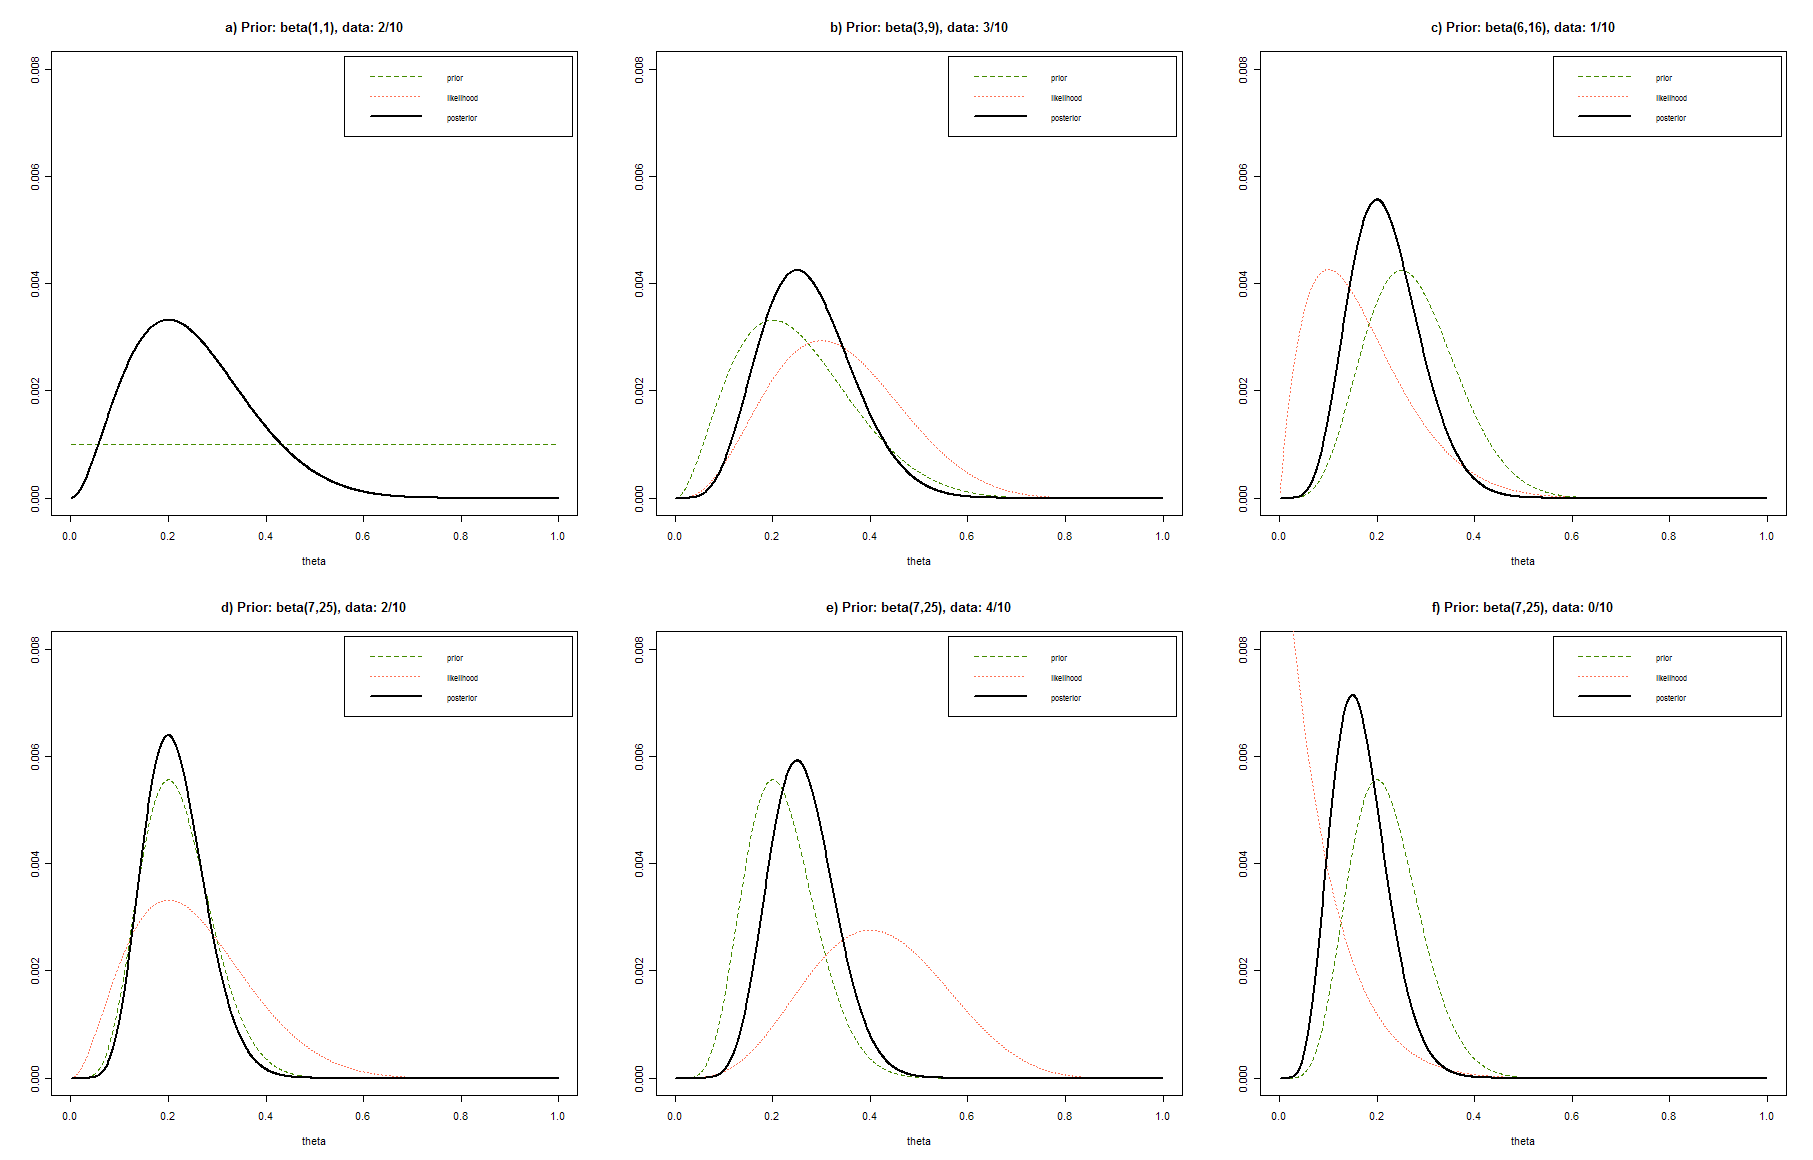
\includegraphics[width=\textwidth]{model-fig-1}
\caption{\textsf{}\label{fig:model-fig-1}}
\end{center}
\end{figure}

Another series of examples is shown in figure \ref{fig:model-fig-2}.  This series of panels shows the same model as above is affected when the prior is changed.  Panel A shows the same result as panels A-D in figure \ref{fig:model-fig-1} where the 40 trials and 8 successes are considered as one set of observations rather than 4 sets of 10 observations.  This illustrates the principle of exchangeability- --the sequence of observations can be changed without changing the results.  Panels B-F show how changing the prior affects the posterior.  Note that in Panel F, even though the initial prior showed a belief in a high probability, the posterior distribution was close to the likelihood.
 
 \begin{figure}[t]
 \begin{center}
 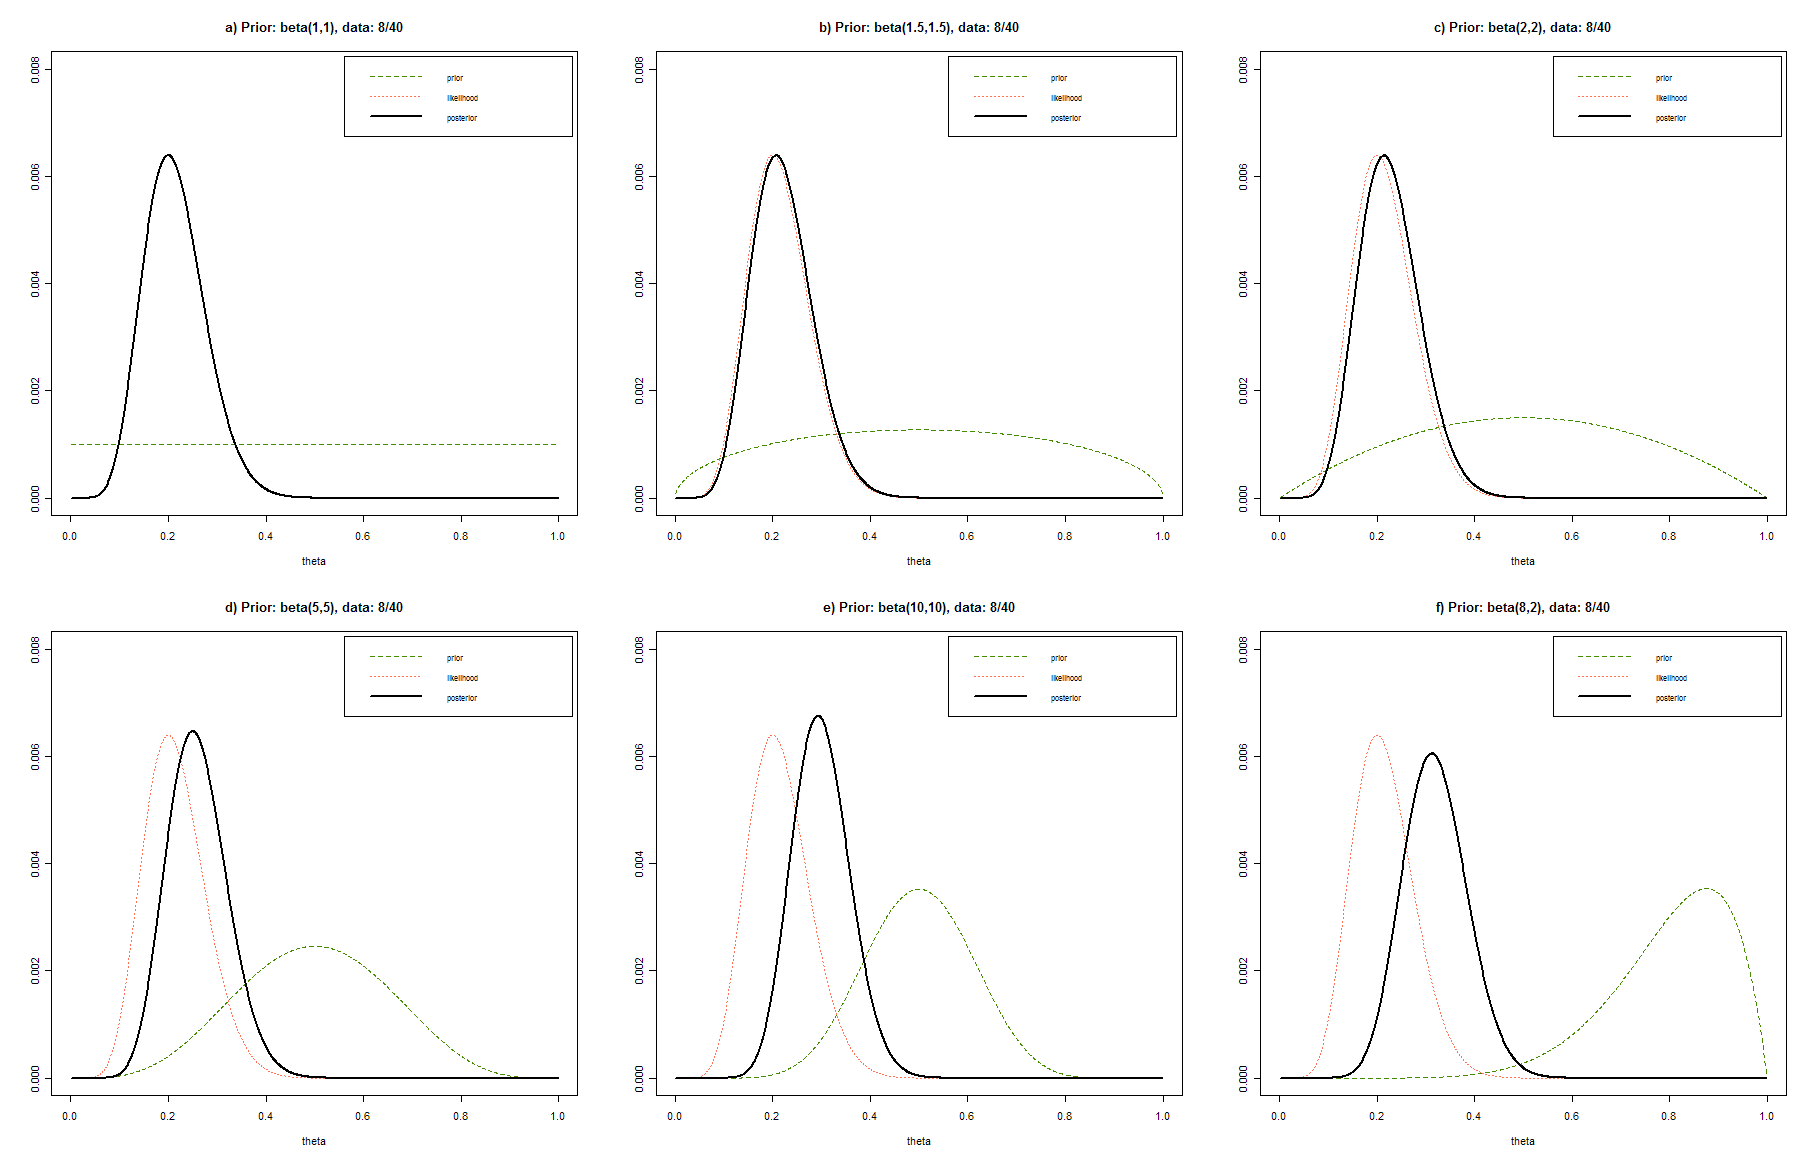
\includegraphics[width=\textwidth]{model-fig-2}
 \caption{\textsf{}\label{fig:model-fig-2}}
 \end{center}
 \end{figure}
 
As these examples show, even when someone who is perfectly Bayesian encounters a set of data that conforms exactly to its true probability, as in the model above, where we sampled 8 successes in 40 when the probability of success was 20\%, their updated belief distribution might still differ significantly from the true probability\footnote{When comparing a single value against a distribution, we can use a measure such as the mean or mode to represent the best estimate based on the distribution.}.   For example, looking at panels D-F in figure \ref{fig:model-fig-2}---the best estimates here differ significantly from the true value---if we had an experiment full of perfect Bayesians with these priors, we would conclude that they significantly overestimated their control!  If we get overestimates of control from perfectly rational Bayesians, then we should reconsider the standard by which we judge participants.

\section{Simulating the Illusion of Control}

We can simulate a standard event-onset experiment as follows: Each simulated participant will observe a number of successes sampled from a binomial distribution, $B \sim (n,p)$, where $n$ is the number of rounds and $p$ is the experimentally determined probability of success.  Each of these participants will have an initial prior belief, modeled by $BE_{prior}(\alpha_{prior},\beta_{prior})$, where $\alpha_{prior}$ and $\beta_{prior}$ are set to reflect the participants initial belief of how likely the button will work.  We can model these Bayesians' beliefs by $BE_{post}(\alpha_{post},\beta_{post})$ where $\alpha_{post} = \alpha_{prior} + $ number of successes and $\beta_{post} = \beta_{prior} +$ number of failures.  We can use $BE_{post}$ to calculate an estimate of the mean for each Bayesian participant by sampling from a normal distribution with the same mean and variance as $BE_{post}$.  Sampling the estimate from this normal distribution gives us estimates that are very close to the beta distribution's mean and introduces some slight variance to allow for frequentist statistical tests.\footnote{The beta variance is very small.}  Finally, these Bayesian estimates can be aggregated and compared to the true probability of the button working through a t--test.  This simulation is repeated 1,000 times to ensure accurate results. From this simulation, we can aggregate the participant's reported mean over all experiments as well as the percentage of the 1,000 simulated experiments that conclude that its participants' means are an unlikely estimate of the true probability.\footnote{This percentage is calculated from the number of experiments that yield a significant t--test that compares the participants' means with the null hypothesis, which is the experimentally determined probability of success, $p$.}

The standard illusion of control experiment gives participants 40 trials to examine the button with half of the trials pressing the button and half not pressing the button.  We can also assume that each condition has 30 participants.  Given that study 2 in chapter \ref{chap:ioc} reported that participants had an average initial belief of success as 45\%, we can set $\alpha_{prior} = 4.5$ and $\beta_{prior} = 10$. Other values of $\alpha_{prior}$ and $\beta_{prior}$ are possible, such as $\alpha_{prior} = 45$ and $\beta_{prior} = 100$ or $\alpha_{prior} = 18$ and $\beta_{prior} = 22$ to represent the expected number of successes over 40 trials. However, increasing the magnitude of the $\alpha_{prior}$ and $\beta_{prior}$ parameters increases the peak of the Beta distribution's curve, effectively increasing the amount of confidence in that particular value. This means that greater weight is placed on the prior compared to the likelihood, which lessens the effect the observed data has on the posterior values. Since these estimates are elicited prior to the experiment, it is unlikely that participants would be tremendously confident in their initial expectation.  Thus, the values chosen for this simulation are conservative estimates, which means that the simulated Bayesians place greater weight on their observations, increasing the probability that their estimates will be accurate.

With these assumptions and parameters we can simulate Bayesian participants testing the efficacious button in the two conditions used in study 3 of chapter \ref{chap:ioc}: The high-control condition's button worked 90\% of the time and the low-control condition's button worked 60\% of the time.  Table \ref{tab:model-results-1} summarizes the results.

\begin{table} 	
	\setlength{\extrarowheight}{4pt}
	\begin{tabulary}{\linewidth}{rcLLL}
	\toprule	
	Condition & \% of Success & Empirical mean estimated contingency & Simulated mean estimated contingency & \% of simulated experiments with significant results\\
	\midrule
	High Control & 90\% & 64.83\% & 65.19\% & 100\%\\ 
	Low Control  & 60\% & 47.00\% & 47.83\% & 100\%\\
	\bottomrule
	\end{tabulary}
	\caption{\textbf{Comparison of Empirical and Simulated Results:} The simulated Bayesians' estimates of contingency are compared to actual experimental results from study 3, chapter \ref{chap:ioc}. The final column shows that every simulated experiment would decide that the simulated Bayesians mis-estimated their control. \label{tab:model-results-1}}
\end{table}

The simulation's results show that perfect Bayesian participants would give results extremely similar to those of the experimental subjects in study 3, chapter \ref{chap:ioc}.  Furthermore, the standard statistical tests used to compare participants' mean estimated control to objective control (i.e. t-tests) of previous research on illusion of control yield a significant result in every simulated experiment!  This result implies that the simulated Bayesians---the normative information processors---have mis-estimated their control!  Perhaps researchers have been too harsh in judgement of their participants and their estimates of control? 

The pattern of results of the Bayesian estimates is significant: when actual control is higher than the initial belief, the Bayesian estimate will be an underestimate. Similarly, when actual control is lower than the initial belief, the Bayesian estimate will be an overestimate. This pattern verifies and provides a more thorough explanation for the process by which participants in the studies in chapter \ref{chap:ioc} arrived at their estimates.

Finally, the number of trials that each participant has to sample the buttons can make a big difference in the accuracy of their estimates. The standard in illusion of control research of giving participants 40 trials means that participants will get little data on the contingency associated with each option. Since increasing the number of rounds raises the risk of fatigue among participants, there is a balance between giving participants enough data and giving them too much. However, these results imply that past experiments have not given participants enough observations.
 
While this simulation suggests that participants should not be faulted for their reported estimates, it still does not address whether participants are aware of the experimenter's normative measure of control, even given their beliefs.  
 
\section{What is the right way to measure control?}

Skinner (1996) suggested a framework for categorizing constructs of control, one dimension of which is particularly relevant to the definition of control given by $\Delta P$: the distinction between the relations of agents, means and ends; in particular: agent-ends and means-ends relations.  A means-ends relation is the connection between particular classes of causes and the set of possible outcomes in a situation (Skinner, 1996) and can be considered the set of contingencies between causes and outcomes. An agent-ends relation is the relationship between a person and the outcomes in a particular situation. Skinner calls this relation the prototypical definition of control. Indeed, under Skinner's framework, the concept of control requires that, ``both objective and subjective control require that two conditions be met: There must be at least one means that is effective in producing a desired outcome... and the individual must have access to that means.'' Thus, the standard definition of control used in illusion of control research and estimates of contingency and means-ends relations in general do not match any of Skinner's definitions of control!  While work has not been done  on surveying the layperson's conception of control, it is reasonable to be doubtful that participants in illusion of control experiments would agree with an experimental measure of control that Skinner classifies as `perceived contingency' rather than true control.

\chapter{Understanding the Meaning of Control}
\label{chap:bioc}

\epigraph{\SingleSpacing The law of causality, I believe, like much that passes muster among philosophers, is a relic of a bygone age, surviving, like the monarchy, only because it is erroneously supposed to do no harm.}{\textit{Selected Papers}\\ \textsc{Bertrand Russell}}

\section{Study Introduction}
\lettrine[lines=2,slope=-3pt,nindent=2pt]{T}{here} are a number of concerns about the results of previous illusion of control experiments.  As demonstrated above, if participants following the normative process for inference are unable to meet the strictures of researchers' tests and their agreement with the normative measure for control is unclear, then more work needs to be done to address the question of how people estimate control.
This study seeks to address some of these concerns by measuring the estimates of contingencies that participants make as they are progressing through an event-onset experiment in addition to collecting their final estimates of contingency and control.  

The central question this study addresses is, ``Do people estimate control using \deltap \xspace as a normative model?'' This study also examines the connection between steps 1 and 2 of the normative model for estimating control in chapter \ref{chap:history}, in other words,  ``How are estimates of the contingency between buttons and outcomes related?''  I consider the possibility that people's estimates of contingency are not systematically biased.  Instead, mis-estimates of control are mainly the result of a disparity between participants' and researchers' definition of control.  A secondary goal of this study is to compare the process by which people process information to a Bayesian process, in an effort to understand the process by which people estimate control.

\section{Method}

\subsection{Participants}
165 participants were recruited online through Amazon's Mechanical Turk and paid \$1.25 for 15 minutes of work.

\subsection{Study Design}

Participants were told they were taking part in an experiment to understand how people estimate control. This experiment used the same basic framework as study 3 in chapter \ref{chap:ioc}, but made several extensive modifications.  Participants were told that they were going to take part in a study about estimating control.  Each round, participants were presented with a choice of pressing one of two buttons, Button A or Button B.  After selecting a button, they would observe whether a light bulb came on.  The experimental instructions told participants that each button had a chance of making the light bulb come on, that these probabilities ranged from 0\% to 100\%, were independent, and would not change during the experiment.

Each button was required to be pressed 50 times (for 100 total times), but the order in which these were pressed was left to each participant.  An on-screen counter kept track of how many times each button was pressed.  Previous experiments on the illusion of control usually employed a different design, with participants experiencing only 40 trials with one button that the participant could choose to press or not press each round (the studies in chapter \ref{chap:ioc}; Thompson et al., 2007; Alloy and Abramson, 1979).  Forcing participants to sample each of the possible options prevents them from gathering unequally sized samples, which would distort perceptions of contingency (see Fielder, 2000).  Matute (1996) observes that people have a tendency to take action when given the chance---if participants are not given a reason, they might oversample by pushing only one of the buttons most of the time. Increasing the sample size to 100 rounds partially addresses concerns that participants are not given enough data to arrive at an accurate estimate of the contingencies between buttons and outcomes.  Using two buttons instead of using one (with the option not to press it) removes a potential confound between taking an action that may generate an outcome and observing an outcome. 

\subsection{Estimating Bayesian Beliefs of Contingency}

Before beginning the experiment and every 10 times a button was pressed, the following procedure elicited participants' beliefs about the contingency of the button and the light. Participants were told, ``We will ask you to estimate the likelihood that pushing Button A (and B) ten times in a row will produce 10 lit bulbs as well as estimating that pressing it ten times will result in 9,8,7,6,5,4,3,2,1 and 0 lit bulbs.  These probabilities should reflect your own personal estimate of the number of times the light bulb would come on, given what you have observed.''\footnote{This elicitation technique is similar to the \emph{hypothetical future sample} (HFS) method described in Garthwaite, Kadane and O'Hagan (2005).} They were shown an annotated version of the tool they would use to give these estimates as well as several examples of sample distributions along with an explanation for what they represent.  Their responses were constrained to a total probability of 100\% for each button.  This procedure was used for each button a total of six times. 

\subsection{Other Measures}

After completing the experimental portion of the experiment, participants were taken to a survey where they were asked to give their best estimate of how many lit light bulbs they would expect from each button if they were pressed 100 times.  To incentivize respondents in being accurate, their responses were compared to the results of a simulation of each button being pressed 100 times.  If both estimated frequencies were with 10 light bulbs of the actual results, then participants received a bonus of \$0.5.  

Participants were asked to give their own definition of control applied to the situation they just experienced and then used this definition to estimate how much control they had in making the light bulb light up, using a scale from 0 to 100, where 0 means no control and 100 means full control. Finally, participants were asked to recall the number of lit light bulbs they saw when pressing each button.  

\subsection{Conditions}

Five conditions were used, which varied the probabilities associated with each button.  For purposes of discussion, Button A will be referred to as the `active' button and Button B will be referred to as the `base-rate' button, but the labels for these buttons were randomized in the actual experiment. 

%\begin{table} 	
%	\setlength{\extrarowheight}{8pt}
%	\begin{tabular}{rp{2.5cm}p{3cm}ll}
%	Condition & Active Button \% of Success & Base Rate Button \% of Success & Control ($\Delta P$) & Reinforcement\\
%	\hline\hline
%	1 & 100\% & 50\% & 50\% & 75\% \\ 
%	2 & 50\%  & 50\% & 0\%  & 50\% \\
%	3 & 100\% & 20\% & 80\% & 60\% \\
%	4 & 20\%  & 20\% & 0\%  & 20\% \\
%	5 & 70\%  & 20\% & 50\% & 45\% \\	
%	\end{tabular}
%	\caption{\textbf{Experimental Conditions:} This is the rest of the caption \label{tab:bioc conditions}}
%\end{table}

%\begin{table} 	
%	\setlength{\extrarowheight}{8pt}
%	\newcolumntype{Y}{>{\small\raggedright\arraybackslash}X}
%	\begin{tabularx}{\linewidth}{YYYYY}
%	\toprule
%	Condition & Active \% of Success & Base Rate \% of Success & Control ($\Delta P$) & Reinforcement\\
%	\midrule
%	1 & 100\% & 50\% & 50\% & 75\% \\ 
%	2 & 50\%  & 50\% & 0\%  & 50\% \\
%	3 & 100\% & 20\% & 80\% & 60\% \\
%	4 & 20\%  & 20\% & 0\%  & 20\% \\
%	5 & 70\%  & 20\% & 50\% & 45\% \\
%	\bottomrule	 	
%	\end{tabularx}
%	\caption{\textbf{Experimental Conditions:} This is the rest of the caption \label{tab:bioc conditions}}
%\end{table}

\begin{table} 	
	\setlength{\extrarowheight}{4pt}
	\begin{tabulary}{\linewidth}{rLLLLL}
	\toprule
	Condition & Active \% of Success & Base Rate \% of Success & Control ($\Delta P$) & Reinforcement & Mean Estimated Control\\
	\midrule
	1 & 100\% & 50\% & 50\% & 75\% & 42.34\%  (35.93)\\ 
	2 & 50\%  & 50\% & 0\%  & 50\% & 24.64\%* (26.13)\\
	3 & 100\% & 20\% & 80\% & 60\% & \mbox{40.25\%* (25.76)}\\
	4 & 20\%  & 20\% & 0\%  & 20\% & 19.21\%* (22.96)\\
	5 & 70\%  & 20\% & 50\% & 45\% & 26.97\%* (27.68)\\
	\bottomrule	 	
	\end{tabulary}
	\caption{\textbf{Experimental Conditions:} This table summarizes the experimental conditions by the percentages of success for each button, the actual control as measured by \deltap \xspace and participants' mean estimated control.  Standard deviations are in parentheses and a ``*'' indicates a significantly different result from the objective control. \label{tab:bioc conditions}}
\end{table}

\section{Results}

\subsection{Estimations of Control}

Participants' estimates of control using the 0 to 100 scale follow the expected pattern: underestimates of control when it is high, and overestimates of control when it is low.  In condition 1, the mean estimated control was 42\% compared to an actual value 50\% (actual values are calculated using $\Delta P$), however this condition was the only one that was not significantly different (M=42.34\%, SD=35.93, t(31) = -1.206, p = .237).  In condition 2, the mean estimated control of 25\% was significantly different to the actual value of 0\%, (M=24.64\%, SD=26.13 , t(38) = 5.889, p < .001). In condition 3, the mean estimated control of 40\% was significantly different to the actual value of 80\%, (M=40.25\%, SD=25.76 , t(35) = -9.258, p < .001). In condition 4, the mean estimated control of 19\% was significantly different to the actual value of 0\%, (M=19.21\%, SD=22.96 , t(28) = 4.505, p < .001).  Finally, in condition 5, the mean estimated control of 27\% was significantly less than the actual value of 50\%, (M=26.97\%, SD=27.68 , t(28) = -4.481, p < .001). These results are summarized in table \ref{tab:bioc conditions}.

While these estimates of control follow the pattern shown in previous work on the illusion of control, when we examine participants' estimates of contingency for the two buttons, a different pattern emerges.  Participants' estimated $\Delta P$ can be calculated as the difference between their estimates of the expected number of success in 100 trials for each button.  When this $\Delta P$ value is compared to the actual control that each participant received (that is, the actual contingencies each participant observed), participants' estimates are considerably more accurate!  In condition 1, the mean estimated $\Delta P$ was 44.91\% compared to an observed $\Delta P$ of 50.56\%, these two were not significantly different ($M_{est} \Delta P =44.91, M_{obs} \Delta P = 50.56\%, t(42.54)=-1.965, p=.05598$).  Similarly in condition 2, participants estimated $\Delta P$ as -4\% compared to an observed $\Delta P$ of -3\% ($M_{est} \Delta P =4.18\%, M_{obs} \Delta P = 3.39\%, t(74.74)=-0.3138, p=.7545$).  Condition 3 was still significant, however, with a mean estimated $\Delta P$ of 60\% compared to an observed $\Delta P$ of 78\% ($M_{est} \Delta P =59.86\%, M_{obs} \Delta P = 77.83\%, t(39.75)=-3.831, p<.001$).  Condition 4 was non-significant, with a mean estimated $\Delta P$ of 1\% compared to an observed $\Delta P$ of 0\% ($M_{est} \Delta P =1.2\%, M_{obs} \Delta P = 0.14\%, t(50.5)=-0.411, p=.6828$).  Finally, condition 5 was also significant, the mean estimated $\Delta P$ was 41\% compared to an observed $\Delta P$ of 52\% ($M_{est} \Delta P =41.48\%, M_{obs} \Delta P = 52.21\%, t(37.88)=-2.599, p=.0133$).  These results do indicate that participants were considerably more accurate at estimating the frequency of success associated with the two buttons than their estimates of control would indicate.  Importantly, participants' estimated $\Delta P$ values (with the exception of condition 1) are significantly different from their estimates of control.  If participants were measuring control by using $\Delta P$ or a similar measure, then we would expect these two measures to be highly correlated.  However, across all five conditions, the correlation between participants' estimates of control and their calculated $\Delta P$ values are non-significant. These results indicate that the methods that participants use to estimate control are of a different kind than the normative method expected by \deltap.

Previous experiments did not record the actual data observed by participants, thus preventing any comparison between participants' estimates of frequency of success with what was actually observed.  The current experimental data enable us to measure how accurate participants actually are via a binomial test comparing the estimated frequency with the actually proportion of successes observed for each button.  If the result is non-significant, then we can infer that the participant's estimate was reasonable.  Out of 165 participants, 110 (or 66\%) were reasonable in their estimates of the frequencies of both of the buttons. It is possible that this group of reasonable estimators would be more likely to be using \deltap \xspace as a method of estimating control; however, correlations between measures of control and \deltap \xspace from estimated frequencies are non-significant.  Further, this group's estimates of control are all significantly different from the normative measure of control, across all five conditions, and follow the same patterns seen for the larger set of data.  Essentially, the only relevant difference between the reasonable and unreasonable estimators is that the former were more accurate in estimating the frequencies of the buttons.\footnote{This type of analysis has interesting philosophical implications as well. The standard analytical model is to compare experimental data to objective, often experimentally manipulated, values. This analysis presupposes a view of truth known as the correspondence theory of truth.  This theory holds that a belief is only true if it ``corresponds'' to reality. For example, in our situation, a participant's estimate of control is only true if it corresponds, or is similar to, the objective value of control, \deltap.  However, there are other theories of truth that are potentially relevant.  The coherence theory of truth holds that a belief is true if it is coherent with the other beliefs held by the reasoner.  I believe that Bayesian inference is an example of this theory.  When a reasoner observes new data, they must adjust their beliefs to ensure that they are now coherent vis-\`{a}-vis the new observations, through Bayesian inference.  Similarly, instead of comparing participants' beliefs solely with an objective reality, we could measure their opinions in a way to check if they are mutually coherent, such as comparing a version of \deltap, calculated from their recalled frequencies, to their estimate of control.} 

\subsection{How Bayesian were Estimates of the Probabilities?}

Before analysing how Bayesian participants were, it is important to check if they understood the Bayesian elicitation procedure.  One way to measure this is by comparing participants' estimated frequencies of success per button with the mode of their final Bayesian elicited probability distributions.  For each button, across all conditions, this comparison showed no significant differences between these two measures.  This indicates that participants were reporting consistent measures using both measures.  

A `perfect Bayesian's' estimates of the probabilities associated with each button can be generated using a technique similar to the one described in the section on Bayesian updating.  The initial prior probability distribution for this perfect Bayesian is set to the same initial prior given by each participant. Thereafter, the perfect Bayesian's estimates are updated by the same data observed by the participant.  A comparison of the final elicited probability distribution can be compared to this perfect Bayesian's estimates for each button.  Table \ref{tab:Bayesian comparison} summarizes the results of this comparison.

\begin{table}[t]
\begin{tabular}{ccccccc}
\toprule
Condition & \multicolumn{3}{c}{Button A Modal \%} & \multicolumn{3}{c}{Button B Modal \%} \\ 
 &  Estimated & Bayesian & Actual & Estimated  & Bayesian & Actual \\ 
\midrule
1 & 85   & 100  & 100 & 47.2 & 51.56 & 50 \\ 
2 & 43.1 & 46.9 & 50  & 48.7 & 48.0  & 50 \\ 
3 & 86.9 & 100  & 100 & 21.4 & 21.7  & 20 \\ 
4 & 17.9 & 18.6 & 20  & 22.4 & 17.6  & 20 \\ 
5 & 57.9 & 71.0 & 71  & 24.1 & 20.3  & 20 \\ 
\bottomrule
\end{tabular} 
\caption{Comparison of Participants and Simulated Bayesians' estimates of button probability of turning on the light.\label{tab:Bayesian comparison}}
\end{table}

As can be seen, the only significant differences between participants' responses and what a perfect Bayesian believes occur when the actual probabilities are rather high and participants fail to update strongly enough, as seen in the difference between Button A's modal percentage in conditions 1,3 and 5.  This conservatism is similar to that found by Ward Edwards (1982; Philips \& Edwards, 1966).  Overall, however, the pattern of results shows that participants' estimates hew close to the estimates expected from a perfect Bayesian.  While these results do not conclusively prove that some form of Bayesian updating was used as the process by which participants processed information, the data suggests that some form of Bayesian updating could be used as a descriptive model for inferential updating of frequencies.

Appendix \ref{app:bayesian} contains figures that compare participants' estimates with a perfect Bayesian counterpart for each interval that estimates were elicited.  These figures show that the adjustments that participants made were strikingly in line with what would be expected from a Bayesian reasoner, with the exception of the already noted difference when a button's true contingency was 100\%.  

\section{Discussion}

The results from this experiment indicate that estimates of control and estimates of contingency are only loosely related, if that.  Given the majority of participants are quite accurate at estimating the frequencies of success they observe, it would be also reasonable to expect that they would be able to take the difference between the two buttons' probabilities of success, thus if participants were using \deltap, or some similar measure, to calculate control, their estimates of control would also be quite accurate.  The lack of correlation between control and contingency estimates, even among the most accurate of estimators, indicates that a very different process is occurring in the estimation of control. 

The definitions of control given by participants imply confusion about what control is and how it should be measured.  Indeed, many participants wrote in the survey that they believed that they had no control over making the light bulb come on because it was all controlled by a computer.  Such concerns imply that their model of control extends beyond a means-ends framework to also include the role of the agent.  They also indicate that participants view the experiment very differently from how the experimenters view it.  For example, if a participant believes that the computer running the experimental program has some control over the outcomes (beyond random number generation), they are indicating that they believe there are additional mechanisms in place that have some control over the light bulb coming on.  Other participants believe that they have control because they can choose which button to press, this implies a theory of control that is agent-means oriented.  

\chapter{Exposing Definitions of Control}
\label{chap:explore}

\section{Study Introduction}
\lettrine[lines=2,slope=-3pt,nindent=2pt]{T}{he} previous study showed that there is a discrepancy between how experimenters and participants define control as well as showing that participants' estimates of contingency and subsequently derived \deltap \xspace are accurate.  However, aspects of the experimental design could have affected the results. When participants were instructed to reconsider their beliefs about the probability of each button every 10 rounds, this encouraged them to recall the previous results and served as a method where they could safely store their beliefs. This could have led to participants being unnaturally accurate in their assessment of the contingency of each button.  Aiding to the unnaturalness, participants were forced to sample each button 50 times.

Suppose these conditions were relaxed and participants were free to sample each button as many (or as few) times as they wished, without the intrusion of the Bayesian elicitation mechanism?  Would their estimates of control and each button's contingency follow similar patterns of results? I hypothesize that the lack of a rigid method forcing participants to update their expectations coupled with a more flexible sampling requirement would reduce the accuracy participants show when recalling the contingency of each button.  Furthermore, I believe that participants will not sample the buttons as often as they were forced to in the previous experiment, thus their estimates of the control will be more regressive (i.e. closer to their original prior) than the estimates of control shown in chapter \ref{chap:bioc}.  

\section{Method}

\subsection{Participants}
138 participants were recruited online through Amazon's Mechanical Turk and paid \$0.75 for 10 minutes of work and given an incentive of \$0.50 for accurately estimating their observed contingencies.

\subsection{Study Design}
The design of this study was identical to the study in chapter \ref{chap:bioc} with several important modifications.  First, the Bayesian elicitation mechanism was removed as was the requirement that participants sample each button 50 times.  Instead, participants were instructed to sample each button as many times as they wished and once they were satisfied, they could choose to proceed to a survey to finish the experiment.  This survey was similar in design to the survey given in chapter \ref{chap:bioc} with the addition of two questions on a new page.  The first new question was phrased as follows: 
\begin{quotation}
One way to measure the amount of control that people have in this situation with the light bulbs is to measure the percentage of times the light bulb comes on when you press Button A and when you press Button B.  The difference between these two percentages is the amount of control your choice of which button to press has on the light bulb. 

For example, from your answers, you would expect Button A to light the light bulb up X\% of the time and Button B to work Y\% of the time.  Thus, according to this measure of control, you would expect to have $(X - Y)\%$ control over making the light bulb light up. 

Do you agree with this definition of control? 
Please use the following scale below to indicate how strongly you agree with this suggested definition of control.
\end{quotation}

Subjects were then presented with a 7-point Likert response scale ranging from ``Strongly Disagree'' to ``Strongly Agree''.

The second question asked participants to choose if they felt their original value of control, this new \deltap \xspace value of control or an entirely new value of control, which they supplied, was a better indication of the amount of control they had during the experiment.

This study also used the same 5 conditions used in chapter \ref{chap:bioc} and listed in table \ref{tab:bioc conditions}.  

\section{Results}
\begin{table}[t] 	
	\begin{tabular}{llllll}
	\toprule
	Condition & Active \%  & Base \%    & Actual               & Participants' & Calculated \\
	          & of Success & of Success & Control ($\Delta P$) & Mean Control  & $\Delta P$ \\
	\midrule
	1 & 100\% & 50\% & 50\% & 63.6\%* & 48.8\% \\ 
	2 & 50\%  & 50\% & 0\%  & 34.7\%* & 2.2\%  \\
	3 & 100\% & 20\% & 80\% & 68.4\%  & 84.1\% \\
	4 & 20\%  & 20\% & 0\%  & 17.3\%* & 1.2\%  \\
	5 & 70\%  & 20\% & 50\% & 28.3\%* & 45.6\% \\	
	\bottomrule
	\end{tabular}
	\caption{\textbf{Summary of Results} Results are broken down by condition, Participants' Mean Control and Calculated \deltap \xspace show experimental results.  An * indicates a result that is significantly different from the experimental value. \label{tab:explore conditions}}
\end{table}

Participants' estimates of means are shown in table \ref{tab:explore conditions}, which summarizes the main results.  As the table shows, participants elicited control was significant in all conditions, except for condition 3, and the means of all conditions followed the same pattern of results as in chapter \ref{chap:bioc}.\footnote{This was given in response to the statement: ``Using your personal definition of control given above, please rate the degree of control your actions had on making the light bulb light up on a scale of 0 to 100, where 0 means no control and 100 mean full control.''} As expected, participants did sample each button fewer times than in the previous experiment, with a mean of 66.5 trials and standard deviation of 68.5. However, the hypothesis that the estimates for control would be more regressive is not supported, for example the estimated control means for conditions 1 and 3 are 63.6\% and 68.4\% respectively, compared to 40\% and 42\% in the previous experiment.  

Importantly, participants' \deltap \xspace calculated from their estimates of the contingency of each button were accurate across all conditions.  This indicates that the accuracy in contingency estimates seen in the previous experiment was not an isolated occurrence and the difference between participants' estimate of control and their calculated \deltap \xspace shows a large gap in their understanding of control as it is defined experimentally.      

When presented with the definition of \deltap, participants' reactions were luke-warm.  Table \ref{tab:agree with deltap} summarizes participants' reactions to \deltap.  The table shows that participants, on average, were not enthusiastic about \deltap \xspace as a measure of control (M=4.6, SD=1.8) and were overwhelmingly inclined to favor their own value of control (67\% in favor of their own value of control).

\begin{table}[t]
	\centering 	
	\begin{tabulary}{\linewidth}{rLL}
	\toprule
	Condition & Mean Agreement     & \% Favoring \\
	          & with \deltap \xspace (SD)  & \deltap \xspace (N)    \\
	\midrule
	1 & 4.5 (2.0) & 17.9\% (5) \\ 
	2 & 4.9 (1.3) & 19.4\% (7) \\
	3 & 4.4 (2.2) & 18.1\% (4) \\
	4 & 5.3 (1.4) & 42.3\% (11)\\
	5 & 3.9 (1.8) & 26.0\% (6) \\	
	\bottomrule
	\end{tabulary}
	\caption{\textbf{Summary of Reactions to Definitions of Control} Results are broken down by condition. Mean agreement is measured on a 7-point Likert scale where 1 = Strongly Disagree, 4 = Neither Agree nor Disagree, 7 = Strongly Agree. Standard deviations are in parentheses in column 2. \label{tab:agree with deltap}}
\end{table}

\section{Discussion}

This experiment confirmed the results of the experiment in chapter \ref{chap:bioc} and showed that participants were not easily convinced that using \deltap \xspace to measure control was a significantly better way.  This is in spite of the fact that participants' \deltap \xspace calculated from their estimated contingencies of the buttons was very accurate.  

These results suggest that the robustness of the results of previous work on the illusion of control were due more to a failure to consider if the normative standards for comparison were compatible with the beliefs of participants than with an underlying bias to overestimate control. These results also suggest that it would be worthwhile to further investigate people's opinions on the validity of \deltap \xspace for measuring control and to explore possible ways to increase its acceptance as a normative measure of control.   

\chapter{Control over Non-Dichotomous Outcomes}
\label{chap:widgets}

\epigraph{\SingleSpacing All alterations take place in conformity with the law of the connection of cause and effect.}{\textit{Critique of Pure Reason}\\ \textsc{Immanuel Kant}}

\section{Study Introduction}
\lettrine[lines=2,slope=-3pt,nindent=2pt]{W}{hile} many events in our lives are dichotomous, like the previous event-onset experiment, we frequently encounter events where the outcomes are not binary, but continuous.  The stocks we follow do not just go up or down, they change by a specific value.  Indeed, many light switches today are not binary, the use of a dimmer allows for very fine-grained adjustments to just how much the light
bulb is on. Previous work on estimating control has not examined such scenarios and indeed, while many experiments in the Human Contingency Learning (HCL) and causality literatures have examine complex situations, they have often focused on situations where the outcomes are binary, such as Baker et al. (1993) or Spellman (1996).  (Baker asked if a tank would reach safety or not, Spellman asked if a plant would flower or not.)
The examination of people's estimates of control in these situations is an important step in the development of theories of how people estimate control.

\subsection{Measuring Control in Non-Dichotomous Situations}

In order to examine control in non-dichotomous situations, our normative measure of control needs to be
extended from the \deltap \xspace formula described earlier.  Recall, that the normative
measure of control in a situation with a binary outcome (either $O=1$ or $O=2$) and one
possible cause, with two possible states ($I=1$ or $I=2$) is calculated by: 

\begin{displaymath}
\Delta P = P(O=1|I=1) - P(O=1|I=2)
\end{displaymath}

However, this measure is insufficient for a situation in which the outcome, $O$, can take more than two possible values because the meaning of success, $O=1$, has not been defined. (In the event-onset paradigm, $O=1$ represents the light bulb coming on.) Consider a situation in which we must evaluate the number of `widgets' being produced by a manufacturing process.  Let us further suppose that we have to use one of two machines, $A$ or $B$, each time we test manufacturing process. We can indicate using machine A in place of $I=1$ and using machine B in place of $I=2$.  $O$, however, must be represented by the set of integers from 0 to some realistic upper bound, e.g. $O=0, O=100, O=333, etc.$ In order to specify our criterion for comparison, we must define a condition, for example, $O \ge 100$. In this example, we would calculate our (differential) control of producing 100 or more widgets using machine A over machine B as:

\begin{displaymath}
\Delta P = P(O \ge 100|A) - P(O \ge 100|B)
\end{displaymath}

If both machines manufacture widgets following the same probability distribution, then \deltap \xspace is $0$, as we would expect in a binary situation where the two causes had the same contingency.  If, however, the machines differed in their production of widgets, we would calculate \deltap \xspace as:\footnote{Where $F_X(x)$ is the cumulative distribution function of X.}

\begin{displaymath}
\Delta P = -F_A(x) - F_B(x) \; \mbox{where} \; F_X(x) = P(X \le x) 
\end{displaymath}

This extension of \deltap, while useful, does not provide an obvious answer for questions like, ``How much control do you have in the production of widgets by choosing Machine A or B?'' In order for extended \deltap \xspace to give an answer for control, we must define a threshold of success. Thus, the question to answer would be specified like this: ``If your goal was to produce 100 or more widgets, how much control did your choice of Machine A vs. B give you in reaching your goal?'' However, it is possible to construct a measure of control that would supply an answer to the former question by quantifying the degree to which one of the machines stochastically dominates the other.
 
While the extended \deltap \xspace is consistent with previous normative measures, incoherence due to a lack of a consistent definitive measure of control might be unsatisfactory.  While it might be possible to calculate such a measure based on the idea of stochastic dominance, it would be unrealistic to expect the average person (or even a statistician!) to readily compute this value. An attractive alternative would be to measure control based on a calculation that compares the outcomes between options, for example, you could take the difference in mean outcomes between options. Thus, the average control one would have using two machines to produce widgets would be a measurement calculated by taking the difference between the average number of widgets produced by each machine. However, an important consideration becomes apparent when considering differences between dichotomous and non-dichotomous.  When outcomes are non-dichotomous, not only do options have an average outcome, but also an associated risk--a range of potential outcomes that can be represented by a measure of dispersion (such as a standard deviation). In a dichotomous situation, if two options have the same contingency, then they can be considered functionally equivalent, but when outcomes are continuous, two options can have the same mean and still differ in the range of possible values they can produce. Ideally, a measure of control would encompass risk as well as expectation. Clarifying the particular type of relational control is one way to address this concern. An estimate of means-end relations control would necessarily exclude an agent's risk-preferences (i.e. preferences for ranges of potential outcomes) but when an individual is evaluating their agent-end control, they are estimating their personal sense of control for control and implicitly using their risk preferences in the calculation.  Thus, for the sake of making comparisons across agents, it is easiest to assume risk-neutral preferences. 

\subsection{Experimental Goals and Predictions}

There are two main goals for this experiment.  The first, exploratory in nature, is to test the generality and robustness of how people estimate control under a new experimental paradigm. Secondly, following previous patterns of results, I hypothesize that participants will over-estimate control when it is low and under-estimate it when it is high. This will be primarily due to the presence of estimates that are outliers that skew the data, but even more fundamentally, I expect that the answers, especially the definitions of control, to reveal a lack of consensus among participants' regarding the normative method to calculate control. Based on the accuracy shown in previous studies, I do not expect these mis-estimates of control to occur because participants were unable to ascertain the distribution of the data they observe. 

\section{Method}

\subsection{Participants}
Ninety-nine participants recruited via Amazon's Mechanical Turk participated in the study for a payment of \$1 for approximately ten minutes work.

\subsection{Design and Procedure}

The experiment consisted of a simulation followed by a survey.  The simulation involved participants assuming the role of a `widget' factory manager who is testing two new widget producing machines, Machine A and Machine B.  Participants were told that they needed to test each machine 50 times and observe how many widgets were produced.  The number of tests was justified to participants because the amount of widgets produced was due to two main factors: the machine itself and the (random) effects from other machines and workers in the factory.

Each round they chose which machine to test; an on-screen counter kept track of how many times each machine was tested.  This design ensured that each
machine was tested an equal number of times, while still giving participants a choice in each round. Ensuring equal sample sizes avoided some of the inferential problems arising from differing sample sizes as discussed by Fiedler (2000). Participants chose a machine by clicking its corresponding button.  After participants completed the simulation, they were taken to a survey which asked them to give their best estimate of the average number of widgets each machine would produce if each were run 100 more times.  They were then asked, ``What are the chances of each machine producing 600 or more widgets on a single run?'' and were instructed to respond on a scale from 0 to 100\% where 0\% means no chance at all and 100\% means every run would certainly produce 600 or more widgets.  Finally, participants were asked to give their personal definition of control applied to the situation they just tested and to use that definition to answer ``How much control of widget production did your choice of Machine A vs. B give you?'' and ``If your goal was to produce 600 or more widgets, how much control did your choice of Machine A vs. B give you in achieving your goal?'' using a scale from 0 to 100\%, where 0\% meant no control over the outcome and 100\% meant total control over the outcome.

\subsection{Independent Variables}

This experiment had two conditions which varied the distribution that was sampled when determining how many widgets were produced.  
In the first, the medium-medium condition, both Machines A and B produced widgets by sampling from a normal distribution, with a mean of 500 widgets and a standard deviation of 100.  In the second, called the high-medium condition, Machine A produced widgets from a normal distribution with a mean of 700 widgets and standard deviation of 100 and Machine B produced widgets from a normal distribution with a mean of 500 widgets and standard deviation of 100 widgets.  The amount of control, as measured by \deltap \xspace in the medium-medium condition is 0, and undefined in the high-medium
condition. When a success threshold of 600 widgets was used, the extended \deltap \xspace gave the medium-medium condition had 0 control and the high-medium condition had 68.3\% control.\footnote{In R, this could be calculated like this: ((1-pnorm(600,700,100)) - (1 - pnorm(600,500,100))} Using the mean-outcome differential measure of control, the medium-medium condition again had 0 control and the high-medium condition had control of 200 widgets. Using the mean-outcome differential measure of control, the medium-medium condition again had 0 control and the high-medium condition had control of 200 widgets.   

\section{Results}

\subsection{Participants' Estimates of Means and Control}

Overall, participants reported accurate mean estimates for the number of widgets produced by each machine in each condition (Condition 1: Machine A M=511.6, SD=96.14, t(57)=0.9205, p=.3612; Machine B M=497.5, SD=79.19, t(57)=-0.2421, p=.9096; Condition 2: Machine A M=671.9,
SD=107.9, t(40)=-1.667, p=.1034; Machine B M=475.9, SD=86.33, t(40)=-1.789, p=.08117). As hypothesized, participants in condition 1 overestimated their control (M=23.9\%, SD=27.83, Wilcoxon V=903, p<.001) when asked to estimate it as a probability. Participants in the High-Medium condition reported a higher level of control (M=39\%, SD=32.8) than those in the medium-medium condition, but as noted above, this measure does not have a normative standard for comparison. It was, however, significantly higher than the mean estimate given in the medium-medium condition (Kruskal-Wallis chi-squared = 4.136, p=.042). When asked to assess their control in producing 600 or more widgets, participants in the medium-medium condition reported an average control of 33.67\% (SD=30.78) which was significantly higher than the normative amount of control, 0\%, that they actually had (Wilcoxon V=1275, p<.001). The high-medium condition participants estimated their control when trying to produce 600 or more widgets at 61\% (SD=30.78), which was not significantly different from the normative value of 68.3\% (Wilcoxon V=355, p=.3309). The latter result is counter to the hypothesized result, which predicts that estimates under high control would be significantly less than the normative measure.  

Estimates of control when producing 600 widgets are significantly greater than estimates of undefined control (Medium-medium condition: Wilcoxon V=218, p<.001; high-medium condition: Wilcoxon V=51.5, p<.001) within both conditions.  While it is possible for the extended \deltap \xspace value to be greater or less than the \deltap \xspace value depending on the value chosen for the criterion of success, these consistent overestimates, together with the other estimates of control indicate a lack of conformity to the normative model of estimating control.

\subsection{Assessing the Mean-Outcome Differential Measure of Control?}

Participant's accuracy in assessing control can be assessed by comparing the difference in means between the difference of the participant's report means for both machines and the difference in the actual means of the machines: (Participant's estimated mean for machine A - Participant's estimated mean for machine B) - (Machine A's actual mean - Machine B's actual mean) = 0.  This comparison is not significantly different from 0 (M=2.22, SD=69.7, t(98)=0.317,p=.7519), reflecting the lack of a consistent bias  in participants' assessment of the output of both machines. (Note that these results include all participants.  When participants whose estimated means of the machines are greater than 100 widgets are removed from the data, the results are even better: M=-1.28, SD=51.56, t(82)=-0.2269, p=.8211.)  A histogram of this measure confirms the advantages of this measure, with a normally distributed pattern of estimates around the mean.  The removal of the bounds of the probability scale and the salience of its midpoint has enabled this measure to avoid the floor, ceiling and regression to the mean effects that might skew participant's estimates of control in this experiment.  

\section{Discussion}

The results of this experiment show, like the previous experiment, that participants' estimates of outcomes are fairly well-calibrated, this implies that the difference between these estimated outcomes is accurate compared to what they observed.   Their estimates of control are radically different from the normative measure of control and coupled with their definitions of control, reveal that their beliefs about control are different from each of the proposed normative measures of control.  However, given that their estimates of the outputs of the two machines are so accurate, it is reasonable to assume that they would be able to take the relatively straightforward difference between these measures as a measure of control if they believed that it was an accurate measure of control. Instead, many participants believed that they had little to no control because they could only choose which machine to use, whereas the output from the machine was not under their control.  This implies a belief of control that fits into an agent-ends relation rather than a means-ends relation. Estimates using the mean-outcome differential measure of control do not show an indication of the illusion of control, indeed, participants were quite accurate in their estimates of control using this measure.  

\chapter{Conclusion}
\label{chap:conclusion}

\epigraph{\SingleSpacing My friend, the panda will never fulfill his destiny, nor you yours until you let go of the illusion of control.}{\textit{Kung Fu Panda}\\ \textsc{Oogway}}


\section{General Discussion}

\lettrine[lines=2,slope=-3pt,nindent=2pt]{T}{he} results of these studies, along with the simulation, question the normative standards used to assess estimates of control in prior research on the illusion of control. The results show that far from being ill-calibrated, participants are quite well-calibrated, so long as the standard used to judge their performance is clear and mutually consensual. Appropriate standards reflect the normative process that is expected to be used rather than just the normative standard for outcomes. This means that the role of prior beliefs in participant's judgments needs to be recognized as well as an understanding of their personal idea of control. While participants' estimates of contingency are accurate, participants' estimates of control reflect a dramatically different definition of control from the experimental normative and their own estimates of contingency. The definitions of control that many participants gave reflected a belief about control that implied that control requires sense of connection and intention between an agent's actions and the outcomes (the two chief elements of Thompson's control heuristic).  While the choice between two options can result in a difference in average outcomes, this type of `control' does not include a role for the agent and thus, many participants reported a feeling of little to no control under an event-onset paradigm. This rejection of having control in these situations agrees with Skinner's assessment that means-ends relations are not about control, but perceived contingency.

These results also raise methodological concerns about prior experiments.  The dramatic disagreement between the normative process for information inference and the normative measure for outcomes means that it is possible that experimental results that involve the types of inferences used in estimating information assimilation are questionable because participants could be following a Bayesian pattern of inference and have not had enough data to arrive at an accurate estimate.  It is possible that differences between actual outcomes and expected outcomes can be due to either faulty inferences or due to proper inferences based on prior beliefs that are sufficiently far away such that the estimate still diverges from the expected accurate outcome.  One way to address, or at least mitigate, this possibility is by increasing the sample sizes that participants observe:  more information given to participants dilutes the effects of prior beliefs.  

\subsection{Where do estimates of control come from?}

The present studies do not provide an explanation for the variability of responses when participants estimate their control.  While these estimates are uncorrelated with estimates of contingency, they do vary systematically in response to experimental manipulations.  For example, the present studies show that increases in \deltap \xspace and the reinforcement rate correspond to increased estimates of control; these results corroborate previous results by Thompson et al. (2004, 2007).  While Thompson suggests the \emph{control heuristic} as an explanation for these results, this does not explain why participants' estimates of control and contingency are uncoupled.  Is there an explanation that can explain both these systematic estimates of control and the uncoupling of control from contingency?

A plausible explanation can be found in the idea of attribute substitution (Kahneman and Frederick, 2002). Kahneman and Frederick argue that when someone is asked a question whose answer entails the use of attributes that are difficult to calculate or measure, they are apt to substitute these difficult values with attributes whose values are easier to access (for example, they come to the mind more readily or there is some correlation between the proper attribute and the substitute attribute). They cite a study by Strack, Martin and Schwarz (1988) where people who were asked ``How happy are you with life in general?'' after being asked ``How many dates did you have last month?'' gave answers that had a correlation of 0.66 but when asked in the reverse order had a negligible correlation.  Since a love life has some bearing on how happy someone is, when people were asked how happy they were with life, the response they had just given about their love life was used in their estimate of overall happiness.  

It is possible that a similar situation is occurring when participants in an event-onset experiment are being asked to estimate how much control they have.  Most people have a vague idea of control that is not as precise as \deltap, in this situation other attributes that are similar to control but easier to estimate can be used.  For instance, when someone is asked to estimate to control, a related value they might consider would be the answer to the question ``How much success did you have?'' or ``How much success are you responsible for?''. Many of the factors that influence the perception of success are the same factors as cited by Thompson's control heuristic, perceptions of intentionality and connection, as well as the more specific conditions cited, such as skill-related factors, success or failure emphasis and need for the outcome (Thompson et al., 1998).

This explanation could be tested in several ways, such as by asking participants ``How much success were your responsible for?'' before or after asking them to estimate their control.  When the success question is asked first, it will have a greater effect (i.e. higher correlation) with their control estimate than when it is asked afterwards.  However, if success is already being used as a proxy, the effect of changing the order of these questions will be suppressed.  An alternative would be to solely ask participants either ``How much success did you have?'' (or were responsible for) or ``How much control did you have?''.  The estimates across groups (holding other factors constant) should be highly correlated, indicating that similar attributes are being used to answer both types of questions.   

\section{Implications for other research}
The intuitive appeal of the illusion of control as well as its applicability to many areas of people's lives, has led to its use as a justification for several other theories and areas of research.  However, given that the results of the present experiments casts doubt on the illusion of control, it is useful to consider how a reconsideration of how people intuitively estimate their control affects these theories.

\subsection{Positive Illusions}
Taylor and Brown (1988) argue that positive illusions about the world, such as the illusion of control, are adaptive. Part of their argument is based on research that has shown that depressed individuals are usually more accurate at estimating their control (such as Abramson \& Alloy, 1981 and Alloy, Abramson \& Viscusi, 1981), thus implying at least a correlation between happiness and positive illusions.  However, as Dykman et. al (1989) have shown, depressed people are also more likely to underestimate their control when they do, in fact, have significant control, implying that they are not necessarily more accurate overall. The results from the present studies show patterns that are similar to both of these results: people can be overly optimistic about their control when it is truly low and unduly pessimistic when it is objectively high. One way to reconcile Taylor and Brown's argument with the current results is to focus on the absolute level of control that people perceive.  In both cases of low and high objective control, participants believe that they do possess at least a moderate amount of control, therefore their actions can affect the outcome of the situation.  Thus, it is possible that it is a belief in possessing some control rather than an over-estimate of control that is necessary for the benefits to mental health that Taylor and Brown attribute to positive illusions. This refinement to Taylor and Brown's model would also allow a role for accuracy of beliefs positively affecting mental health, so even greater benefits are accrued to those who believe they have at least a moderate amount of control and are accurate in their estimation compared to those whose beliefs are merely over-estimates of their control.  

\subsection{Overconfidence}
Recent work on overconfidence (e.g. Moore \& Healy, 2008) has shown how situations can be manipulated to encourage people to be either under or over-confident.  For example, people are likely to overestimate their performance on difficult tasks, yet they are also likely to underestimate their performance on easy tasks.  This pattern is similar to the illusion of control results, where situations with low control are analogous to difficult tasks (e.g. the light bulb has a low probability of coming on or the quiz question is unlikely to be correctly answered) and situations with high control are analogous to easy tasks (e.g. the light bulb has a high probability of coming on or the quiz question is likely to be correctly answered).\footnote{It should also be noted that the absolute probabilities for each button making the light bulb light up, and thus, the overall reinforcement rate, will also a play an important role in these analogies. The difficult situation should have a low overall reinforcement rate as well as a low \deltap \xspace value, similarly, the easy situation should have a high overall reinforcement rate and high \deltap \xspace value.} The Bayesian model that Moore and Healy propose for modeling overconfidence is similar to the Bayesian model simulated in Chapter 3 and tested in Chapter 4: people incorporate both their prior beliefs and new evidence when generating a estimate of performance or control.  Indeed, estimates of control could be considered to be indicators of confidence in how much an individual's choices affect the outcome.  The parallels between estimates of confidence and control as well as the models to describe them (and also similar patterns of results) indicates that these concepts are potentially intertwined.  Examining the relationship between control and confidence could be a fruitful area of future research.

\subsection{Power}
The similarities between the definition of control as defined by \deltap \xspace and Emerson's (1962) definition of power are interesting.  Emerson defined power in terms of the relationship between two actors, \emph{A} and \emph{B}.  The power of B over A is equal to the dependency of A on B, where dependency is partly specified as ``inversely proportional to the \emph{availability} of those goals to A outside of the A-B relation.''  Thus, dependency between two actors with respect to a goal is measured by the relative difference in attaining that goal through the relationship compared to other alternatives. Thus, the greater the relative cost to A of pursuing a goal via means outside of the relationship A-B, the greater the dependency of A on B and thus, the greater the power of B over A.  Similarly, control, in the simplest case of two actions, is defined as the difference in probability of an outcome given either action.  Both power and control are defined by the difference (of cost or likelihood) between one alternative and another.  Since power and control are similarly defined, perhaps perceptions of power are affected are affected similar factors as control.  For example, consider an actor in a brokerage role connecting two disparate networks.  How aware are they of their position in the networks?  Does their definition of power match Emerson's definition or does it reflect a different understanding of power, in a manner similar to the behavior of participants in the studies reported in this dissertation?

\section{Limitations of the present work and directions for future research}
The studies in this paper are based of the paradigm originally developed by Jenkins and Ward (1965) and adopted by illusion of control researchers such as Alloy and Abramson (1979).  This design allows for a clarity of presentation and analysis as well as ease of comparison to results from previous studies, but at the expense of unnaturalness.  The ability to rapidly select and observe the unequivocal outcomes of various actions is an unusual scenario that people are unlikely to experience in the real world.  It is possible that many real world factors outside of this paradigm will significantly affect peoples' judgements of control. For example, people are unlikely to press a button at a cross-walk more than a few times a day and each time they do press the cross-walk button, they will have to wait to observe the result. Finally, because the scenarios tested in this paper are artificial, their applicability to the real world and especially the domain of organizational behavior is limited. It is also possible that people are far more observant and accurate when the decisions they are making are of greater consequence, such as in a business setting, they might even employ a different model of control in such a situation.

While these limitations and concerns are significant, the present work should be viewed as a stepping stone towards a greater understanding of control.  As shown above, control as a concept is linked to and similar to several other important concepts, such as power and confidence, and the interplay between these ideas raises many intriguing possibilities for future work.  For example, do people in situations of lower power overestimate their power?  Do they underestimate their power when it is high?  How are perceptions of confidence and control related?  These studies could be extended to situations where people are dealing with others rather than inanimate objects such as light bulbs, such as decision-making in groups or negotiations.  Since people underestimate control when it is high, they might also underestimate their ability to complete tasks on time when their control over these tasks is high.  This could lead to situations where the planning fallacy is reversed.  

Another fertile area is ethics.  Many ethical studies and dilemmas portray actors as having full control and determination over outcomes.  For example, in the popular trolley problem (Foot, 1978), the effect of pushing someone in front of the train is stated with certainty- ``if you push them in front of the trolley, it will stop''.\footnote{A common version of the trolley problem is thus: ``As before, a trolley is hurtling down a track towards five people. You are on a bridge under which it will pass, and you can stop it by dropping a heavy weight in front of it. As it happens, there is a very fat man next to you - your only way to stop the trolley is to push him over the bridge and onto the track, killing him to save five. Should you proceed?'' (Thomson, 1976)}  The probability of this outcome and other alternatives could be varied, thus also varying the control that the actor has on the situation.  It is possible that people think modally (as modal logic) when considering these decisions, even if not explicitly instructed to, for example, even if told that pushing the fat man \emph{will} derail the trolley, the realistic uncertainty of the outcome of such an action might factor in the decision-making process and affect a person's choice in whether to push the man off or not.  Varying the control people have in this dilemma would make these situations more realistic and by making these potential unstated factors explicit.  Would you push the fat man off if the chance of derailing the trolley was only 50\%?  

More fundamental research could manipulate the prior beliefs of participants and reasoning under experimentally manipulated priors to examine the methods of information assimilation used when priors are extrinsic.  

The results in chapters \ref{chap:bioc} and \ref{chap:explore} suggest that people are resistant to \deltap \xspace as a normative measure of control.  Further work could investigate why this is so and explore possible ways of increasing agreement with its use as a normative measure.  


\section{Reconsidering the Nature of Control}

Most of the definitions of control given here and elsewhere imply that control is a probability.  For example, Bandura (1977) described control as, ``one's estimate that a given behavior will lead to certain outcomes'' and Heckhausen (1977) gave, ``the subjective probability that one's actions will modify a given situation'' as a definition.  However, it might be more useful to think about control in terms of causation rather than as a probabilistic measure.  Consider the common statistical epigram, ``correlation does not imply causation'' applied to the above definitions.  When control is measured as the difference in probabilities, what is being measured is the difference in correlations rather than actual causation. The definitions given by Bandura and Heckhausen imply that an aspect of causation is essential to the judgement of control, for example, to use Heckhausen's definition, one's actions will modify a situation by causing some effect. Thompson's control heuristic reflects this desire for an awareness of causality.  I become more certain about my role as the causal agent in a situation when I intend to perform an action (intentionality) and I feel that my action was necessary for the action to occur (connection).\footnote{This re-conception of control also implies that greater precision in predicting the outcome will increase my estimate of control.} This re-conception of control can explain why higher reinforcement rates in event-onset experiments increases estimates of control (Thompson, Armstrong, \& Thomas, 1998) .  Higher reinforcement implies more certainty that an action (in fact, any action) will lead to an expected outcome.  While the difference in contingencies among possible choices can reflect differential control, overall control could be measured as some aggregate function over the set of options.  For example, consider two parallel situations in an event-onset experiment.  In the first situation, I have two buttons, each of which has a 100\% of making a light come on.  In the second, I also have two buttons, but each of these has a 0\% of making the light come on.  According to the \deltap \xspace measure of control, the amount of control in both situations is zero.  However, there is a distinct difference between these two situations.  In the second, no matter what I do, that light will not come on.  In first, that light will come on, when and if and only if, I push a button.  If I get up and walk away, that light will still be off when I return. While my differential control, measured by \deltap, between options in my choice set might be zero, I still am the cause (and the apparent only possible cause) of the light coming on.  Thus, it is reasonable to conclude that my control in the first situation is quite high. This explanation entails that participants view the scope of the experiment differently from the experimenters.  For example, Alloy and Abramson (1979) touch on this idea when they explain a potential problem with how participants might have viewed Jenkins and Ward's (1965) experiments.  These experiments had subject choosing to press one of two buttons, but since each round was self-initiated, participants might have been evaluating three possible causes---button one, button two and no button at all.  If they were, Alloy and Abramson state that they would justified in judging control based on how much success they had when pressing a button.

\section{Conclusion} 
The results of the studies in this dissertation reveal that the illusion of control, along with mis-estimates of control in general, appears to be an illusion itself due to a lack of common understanding of how control should be calculated. These results are replicated across several different paradigms and appear to be robust.  Additionally, these studies reveal methodological issues with previous work on the illusion of control and suggest that greater care needs to be taken when examining concepts whose measurement is not obvious. So are people's estimates of control accurate? My work shows that, yes, people are accurate when they estimate control, but only if you ask them properly.

\appendix
\chapter{Instructions used in Study 1, Chapter \ref{chap:ioc}}
\label{app:study-1-instructions}
ATTENTION AND VISUAL PERCEPTION

In this experiment, we are interested in understanding the impact of distractions on visual perception. You will play 10 rounds of the same game.  

In each round, you will be presented with a screen full of letters in random sequence. 

Your goal in each round is to find all the instances of two same consecutive letters (for example ``g g'' or ``r r''). Click on the letters with the mouse to get them to count.  Each round will last for 90 seconds.

Every few seconds, the colors on your screen may change: from black ink on white page it changes to violet ink on black page. 

There is a button on the screen that says ``STAY WHITE''. The button will appear on the top left corner of your computer screen.  

You can press this button only once in every five-second interval.

Pressing the ``STAY WHITE'' button may help keep the screen white. If it works, then the screen will stay white with blank ink for the remainder of the 5-second interval.
 
To start the experiment, press the ``CONTINUE'' button below.

Good luck!

\clearpage

\chapter{Contingency Learning: Participants vs. Bayesian}
\label{app:bayesian}

This appendix presents five figures that compare the estimates of participants from chapter \ref{chap:bioc} to a perfect Bayesian reasoner.  The values shown are the mean of the elicited estimates at the start of the experiment and every time a button was pressed ten times.  The values for the Bayesian reasoners show the same initial value as the participants, thereafter, the Bayesian values are generated by Bayesian inference over the same likelihood values as the participants saw. The error bars show the standard error (which in some cases is too small to be shown). 

These figures show participants' estimates were extremely similar in direction and magnitude to their equivalent Bayesian counterparts.  

\begin{figure}
\begin{center}
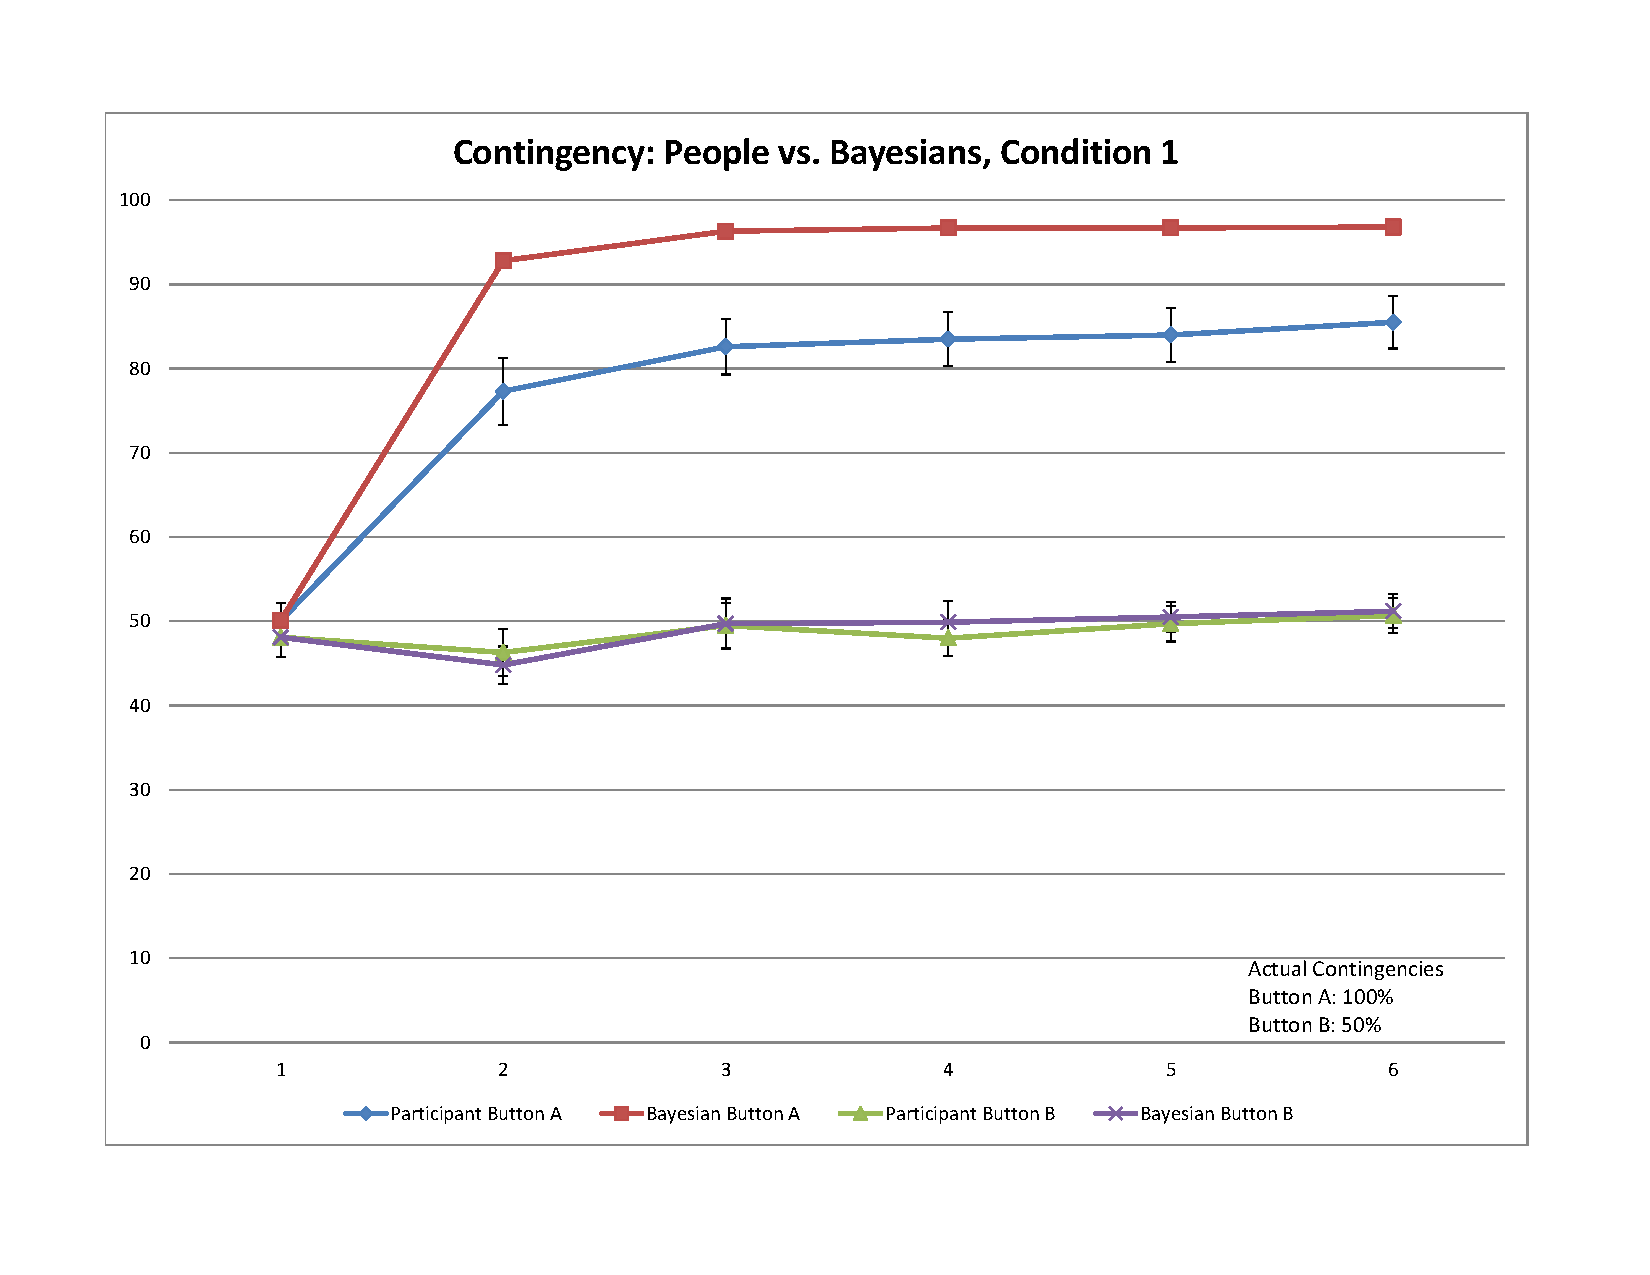
\includegraphics[width=\textwidth]{learning1}
\caption{\textsf{}\label{fig:learning1}}
\end{center}
\end{figure}
 
 
\begin{figure}
\begin{center}
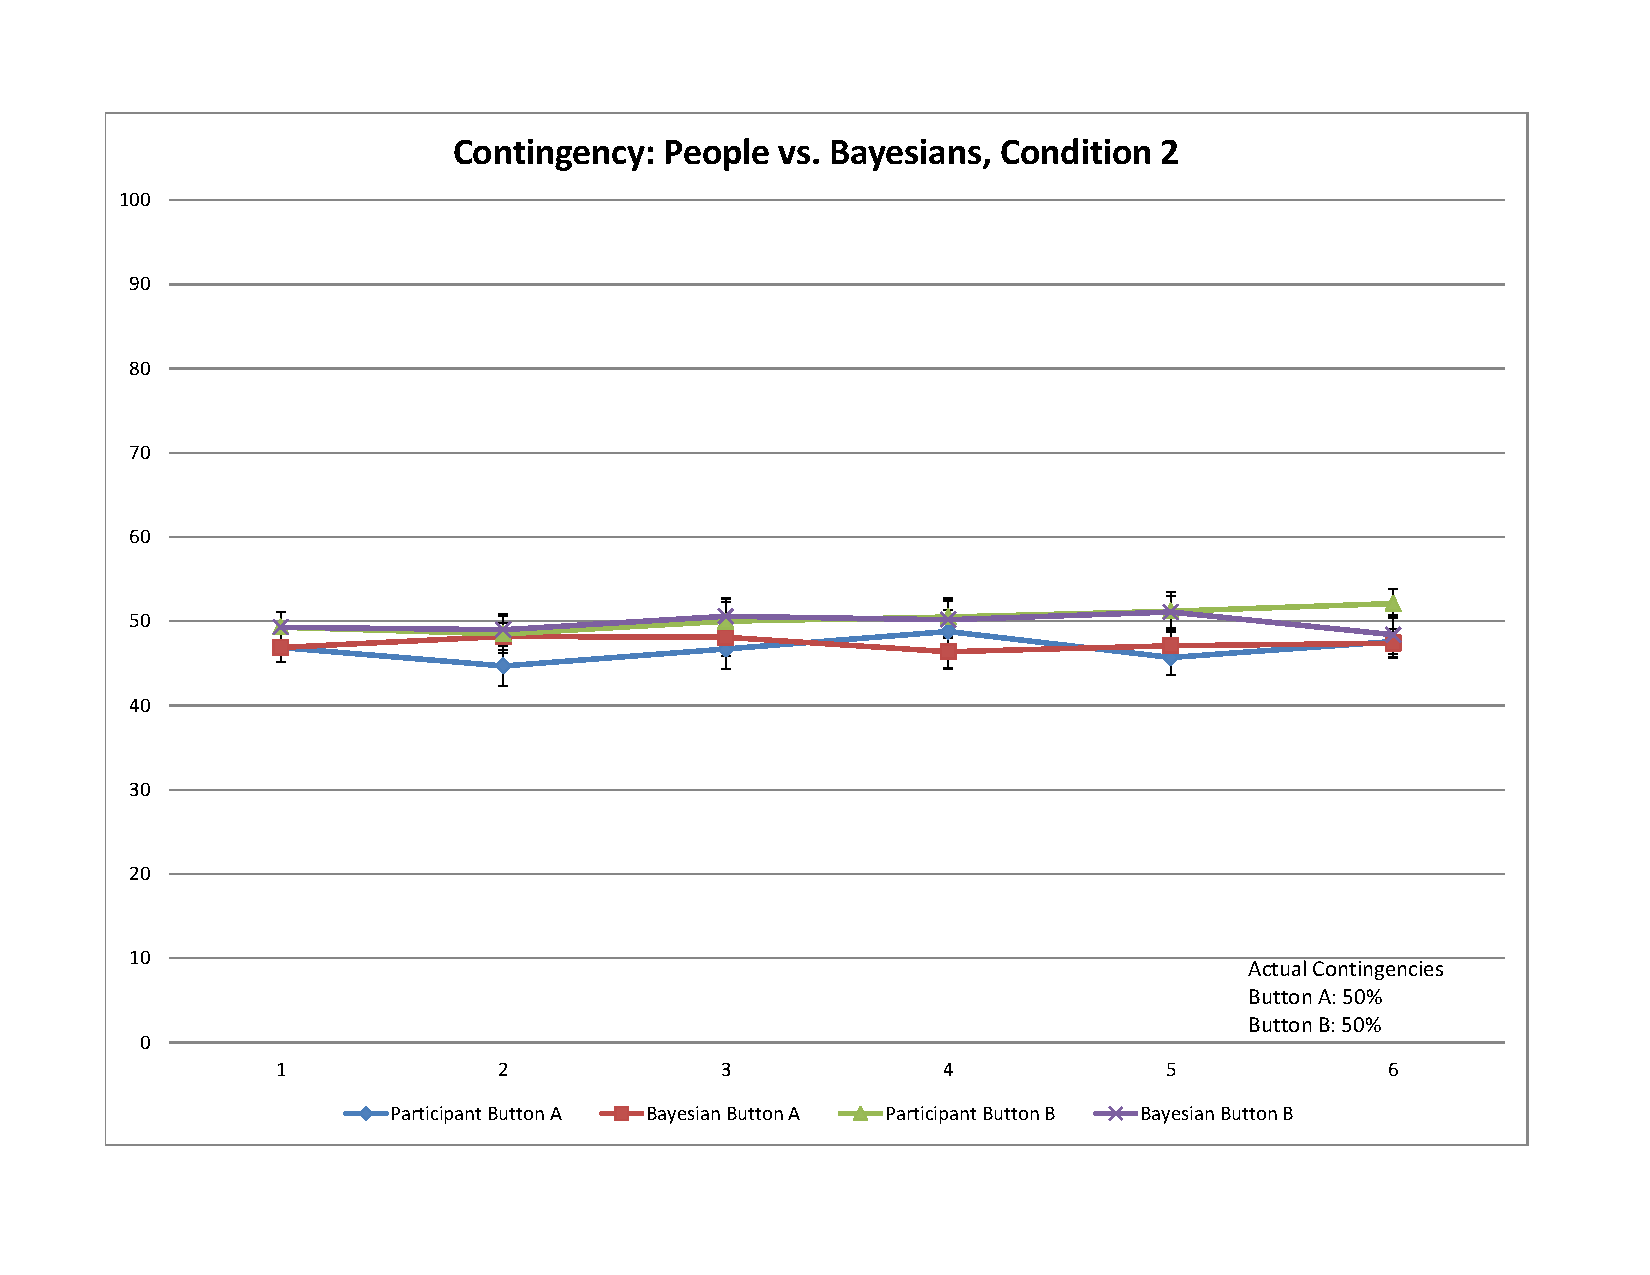
\includegraphics[width=\textwidth]{learning2}
\caption{\textsf{}\label{fig:learning2}}
\end{center}
\end{figure}
  
  
\begin{figure}
\begin{center}
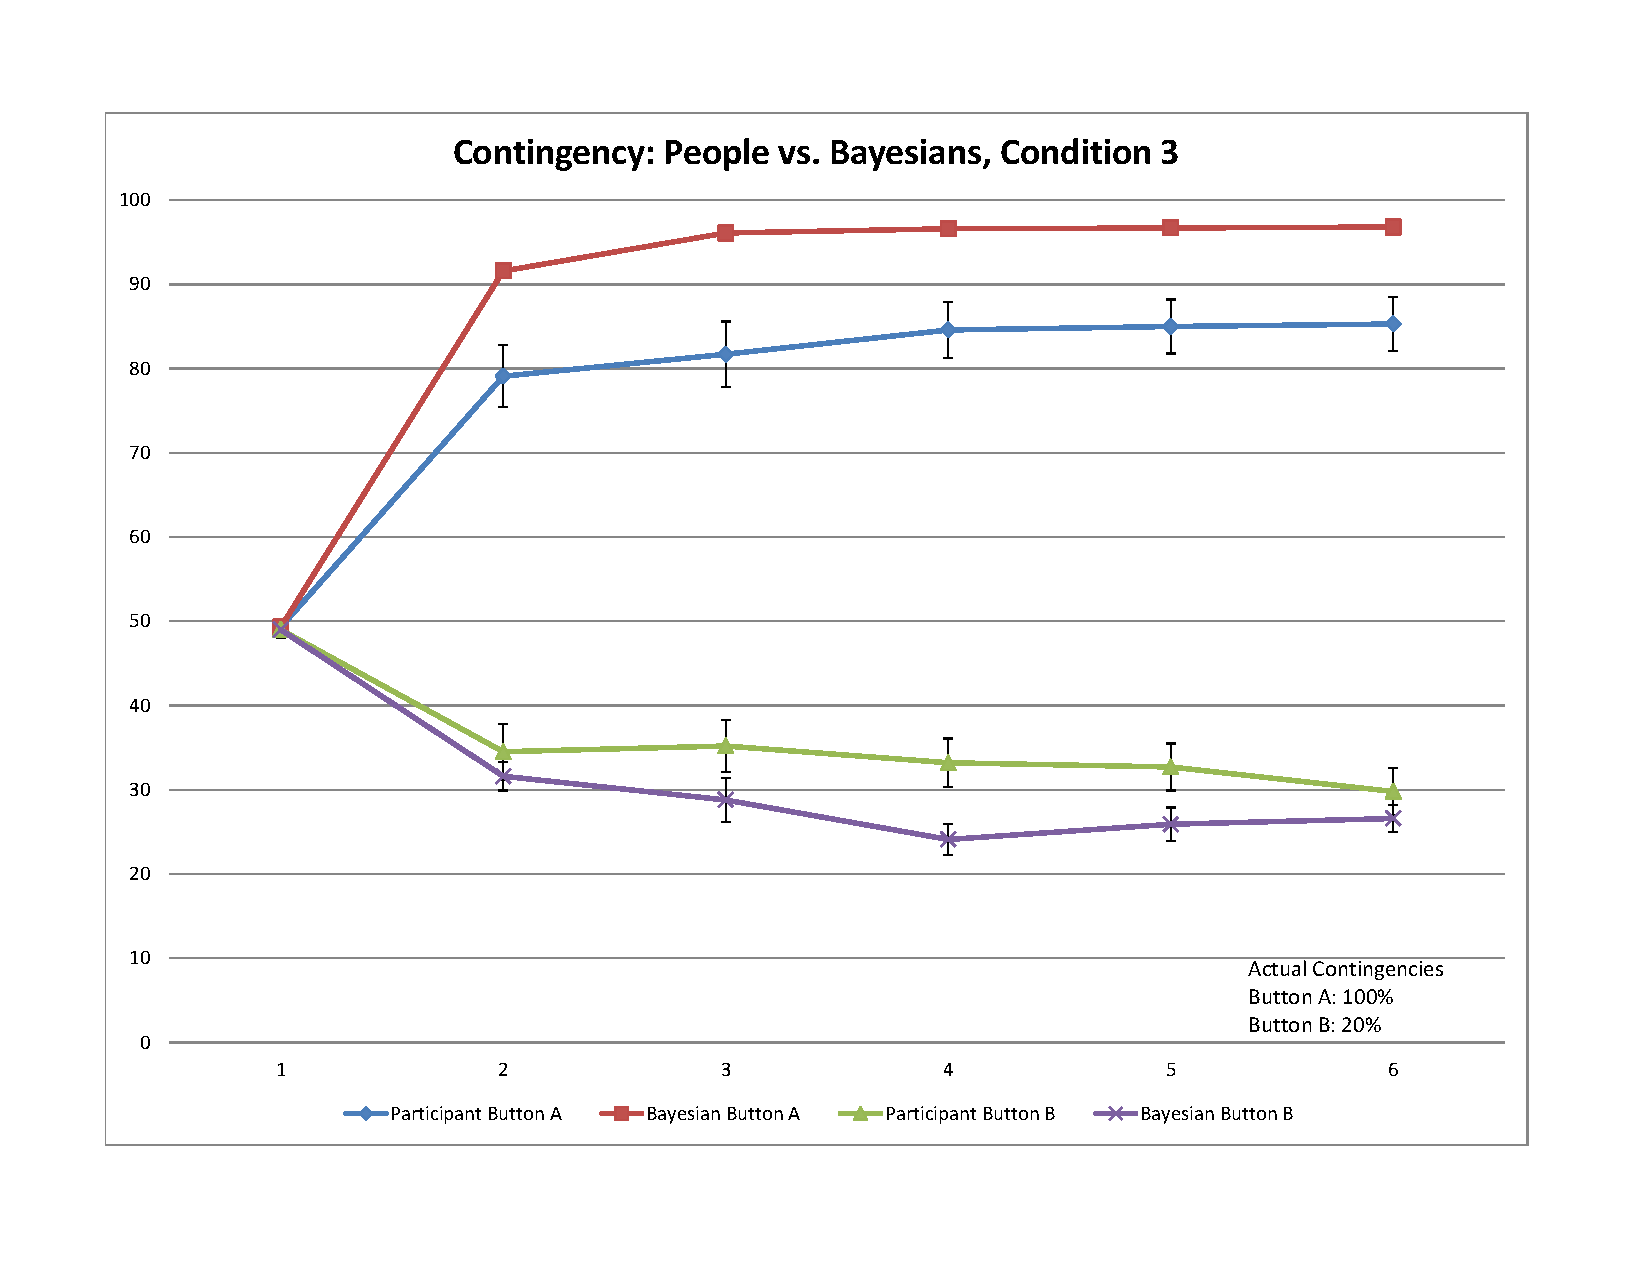
\includegraphics[width=\textwidth]{learning3}
\caption{\textsf{}\label{fig:learning3}}
\end{center}
\end{figure}

\begin{figure}
\begin{center}
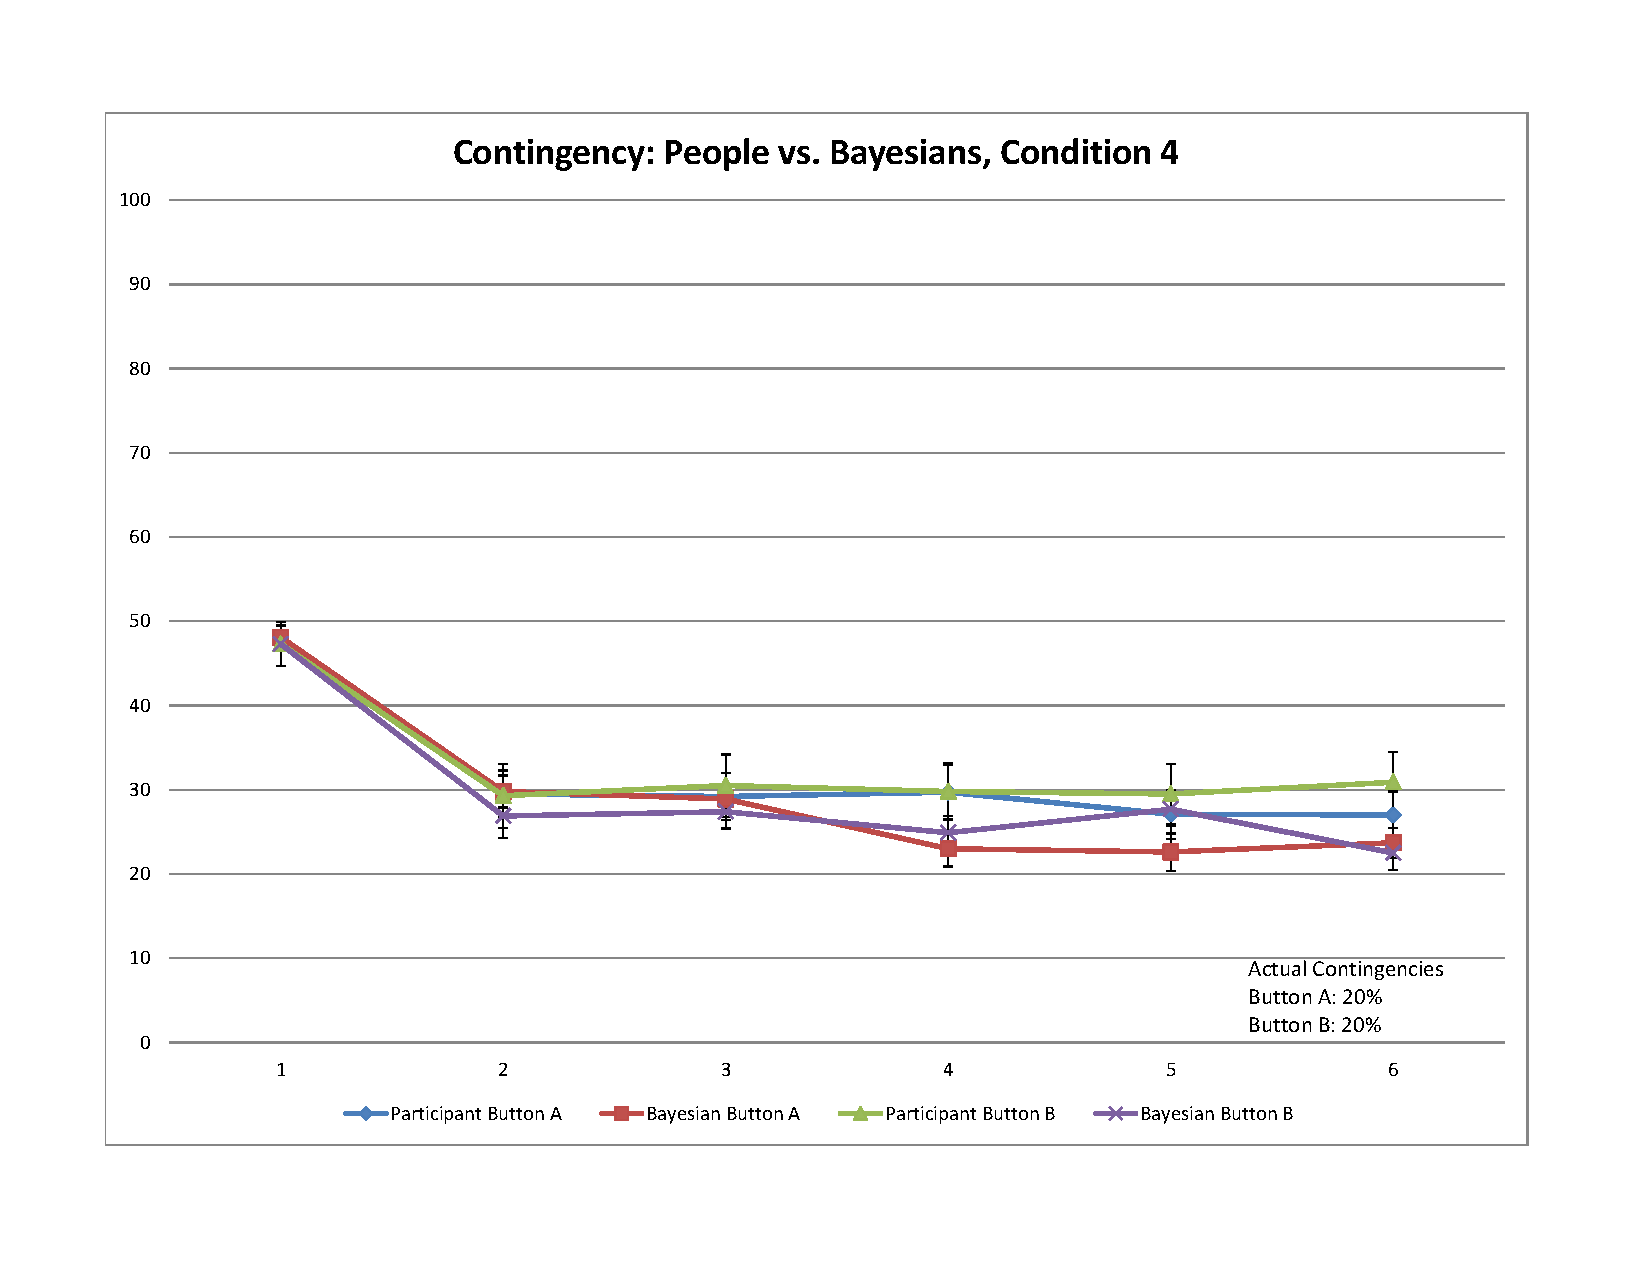
\includegraphics[width=\textwidth]{learning4}
\caption{\textsf{}\label{fig:learning4}}
\end{center}
\end{figure}
 
\begin{figure}
\begin{center}
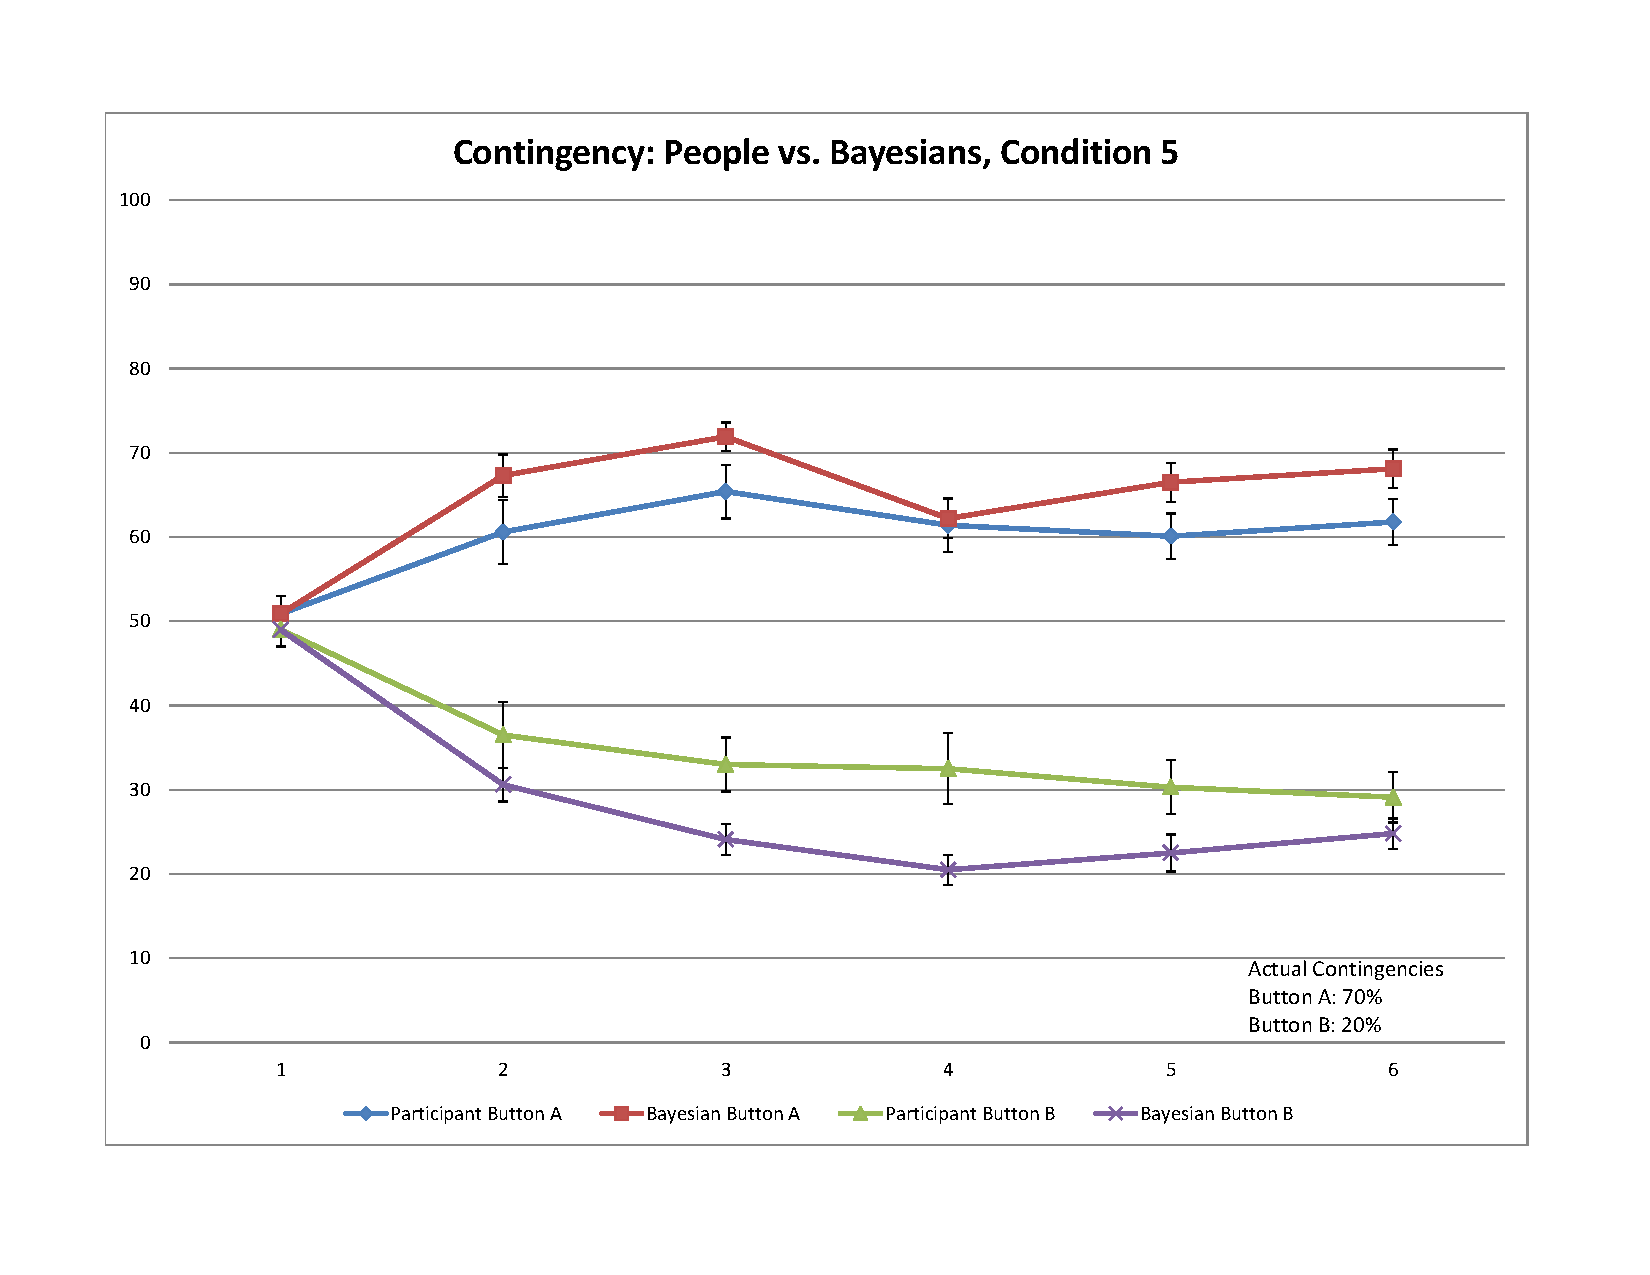
\includegraphics[width=\textwidth]{learning5}
\caption{\textsf{}\label{fig:learning5}}
\end{center}
\end{figure}
 

\backmatter

\bibliographystyle{apacite}
\bibliography{dissertation-references}
\nocite{*}

\chapter{Colophon}

This document was created with the \LaTeXe \xspace typesetting system using the Adobe type faces Minion Pro for the main text and Myriad Pro for sans-serif text. The layout was inspired by Robert Bringhurst's \textit{The Elements of Typographic Style}. 

The experimental data was analyzed using the R programming language; both the raw data and code are available from the author at sharek@gmail.com.
\vspace{3cm}

\centering{\Huge\ding{166}}


%
\end{document}



